\section{Experiment 1: Feature Extraction}
The python version CIFAR10 and CIFAR100 datasets are downloaded from the official website with pre-defined train and test sets. The train set were split into train and validation sets with the ratio 8:2 randomly. We got 40,000 train samples, 10,000 validation samples and 10,000 test samples for both datasets. In order to speed up the experiments, we started by extracting the image feature vectors with a single forward propagation before training the FC layers.

All trainable parameters of the two FC layers were initialised by the Xavier uniform method \cite{Glorot2010}. The training process was monitored by the validation accuracy. After each epoch, we reported the validation accuracy and kept a record of the model parameters which achieved the best validation accuracy so far. We scheduled two training stages to approach the optimal classification accuracy. First we performed 500 training epochs with step size 0.01 then decreased it to 0.001 for another 500 epochs.  After each training stage, the recorded parameters were loaded to prevent overfitting. The final held-out test set accuracy for CIFAR10 is 0.9258 and for CIFAR100 is 0.7444. Finally we compressed the extracted 4032-D feature vectors with the 128-D FC layer.

We further took a closer look at the compressed features by projecting them down to two dimensional vectors with t-SNE \cite{Maaten2008} and maintains the relative distance between samples. The plots are shown in Figure \ref{Fig.tsne}. Different colours represent different classes of samples. First of all, the network transformed the images into blobs where ideally samples from the same class should be closer to each other. This is true especially for CIFAR10. The quality of these compact blobs reflects the classification accuracy. Strays far from the cluster would be misclassified by the logistic regression layer thus lower the classification accuracy. Furthermore, the boundaries between different classes are not always clear. Blobs are close to each other near the boundary thus the classification accuracy is sensitive to slight variations of the boundary. The effect is more obvious if there are more samples for each class. This partly explains the rapid vibration of the CIFAR10 validation accuracy curve shown in Figure \ref{Fig.extracthis.a1}. In fact, we can widen the distance between adjacent blobs by fine-tuning the pre-trained feature extraction network and achieve a higher classification score \cite{Kornblith2018}. However, since we want to minimise the pre-processing time required, we omitted this step and stayed with the sub-optimal features.


\begin{figure}[H]
\centering  
\subfigure[CIFAR10]{
\label{Fig.sub.a1}
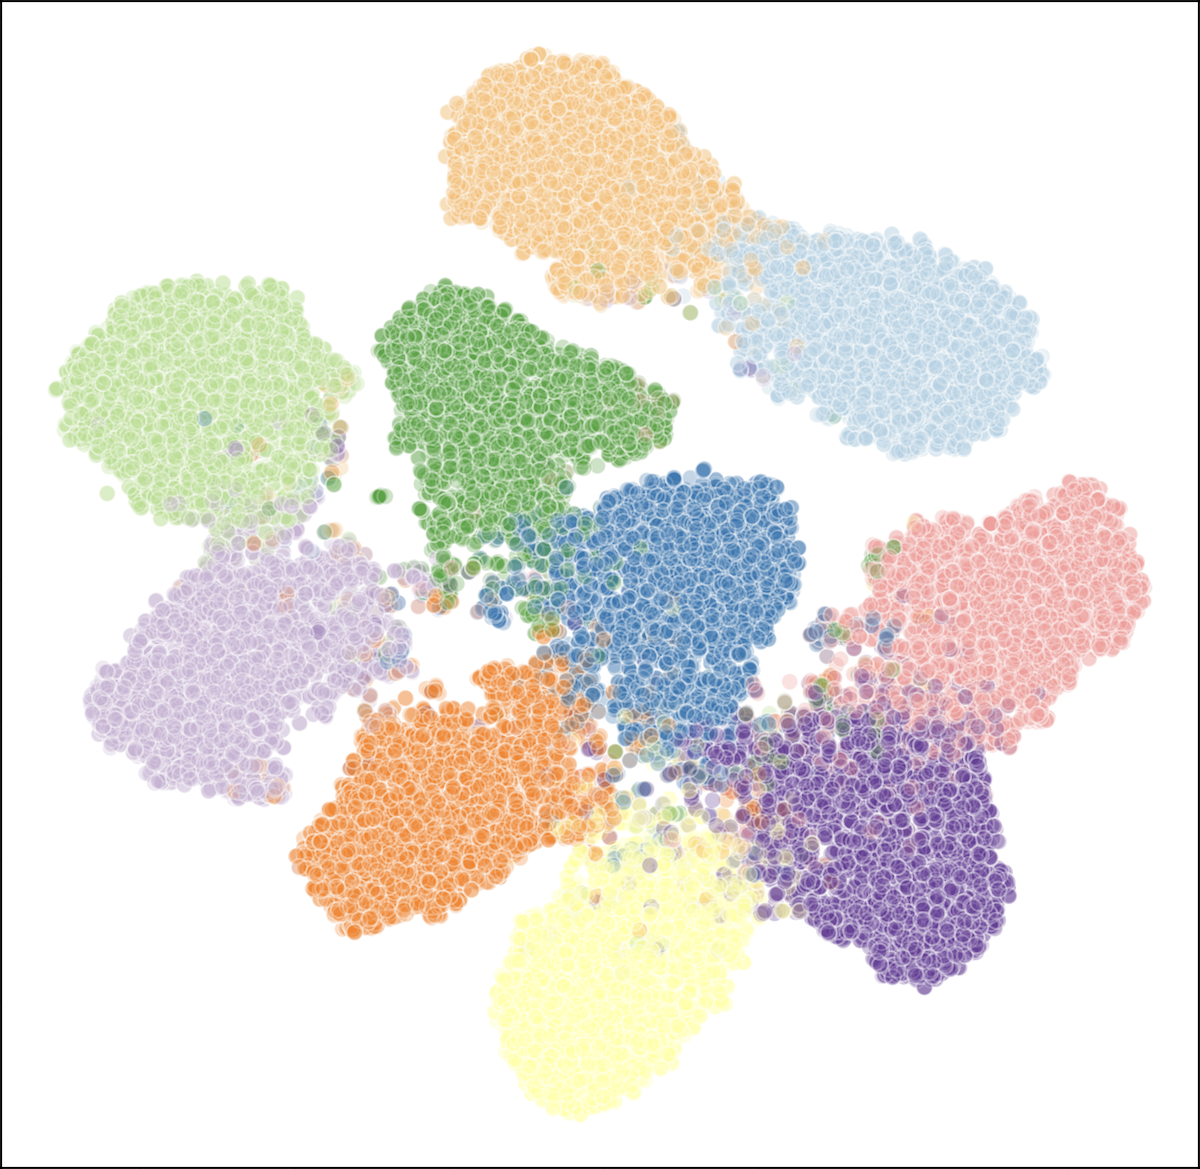
\includegraphics[width=0.45\textwidth]{src/cifar10-tsne.png}}
\subfigure[CIFAR100]{
\label{Fig.sub.a2}
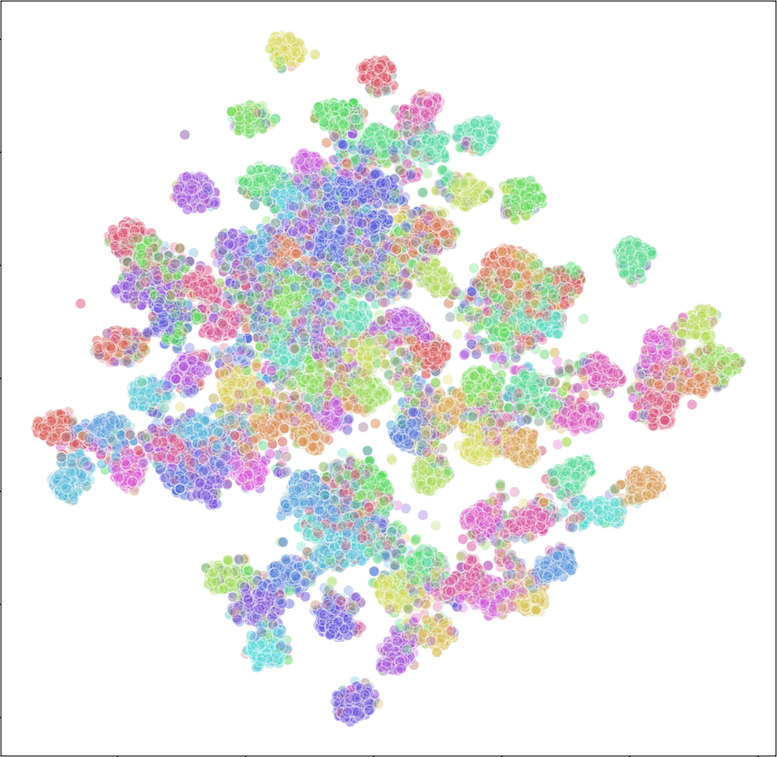
\includegraphics[width=0.45\textwidth]{src/cifar100-tsne.png}}
\caption{Visualisation of extracted features with the t-SNE algorithm.}
\label{Fig.tsne}
\end{figure}

In addition, we compared the training process of the two datasets in Figure \ref{Fig.extracthis}. Across the two training stages, CIFAR10 converges faster than CIFAR100 but it starts to overfit earlier. The green line indicates that we could reduce the number of epochs in the first training stage by half and leave the mining job at the second  stage. 

Finally, we also visualised the classification distributions in Figure \ref{Fig.clscores}. As observed from the quality of blobs plotted in Figure \ref{Fig.tsne}, CIFAR10 samples tend to achieve higher classification scores around 0.9 while CIFAR100 samples are spread across the range below score 0.9. Samples from CIFAR100 are harder to classify correctly with lower scores. Based on the sample selection procedures described in Chapter \ref{bg}, we may need more samples for CIFAR100 to achieve a similar relative accuracy compared with CIFAR10. This suggests that data reduction algorithms may be less efficient for datasets with more classes and lower classification accuracy. We will discuss the algorithm performance further in Section \ref{lr} and \ref{CNN}. 

\begin{figure}[H]
\centering  
\subfigure[CIFAR10]{
\label{Fig.extracthis.a1}
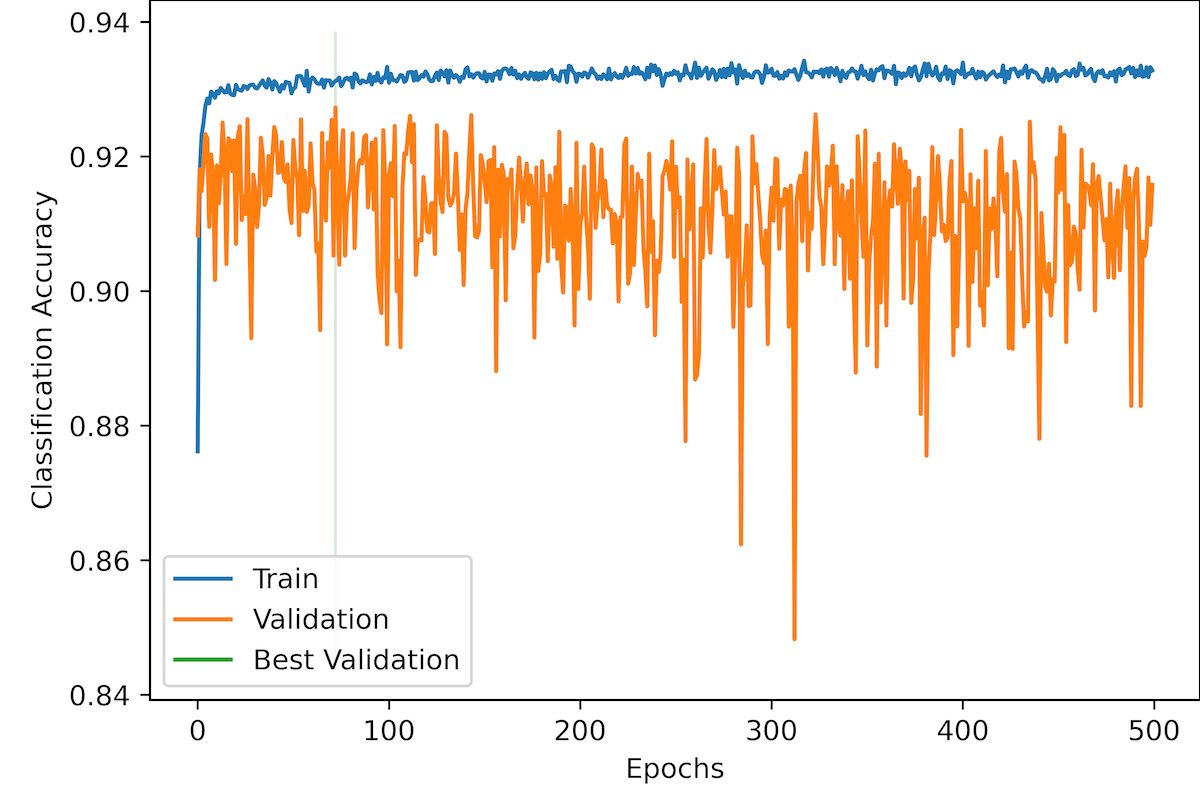
\includegraphics[width=0.45\textwidth]{src/cifar10_exp1_train.png}}
\subfigure[CIFAR10]{
\label{Fig.sub.a2}
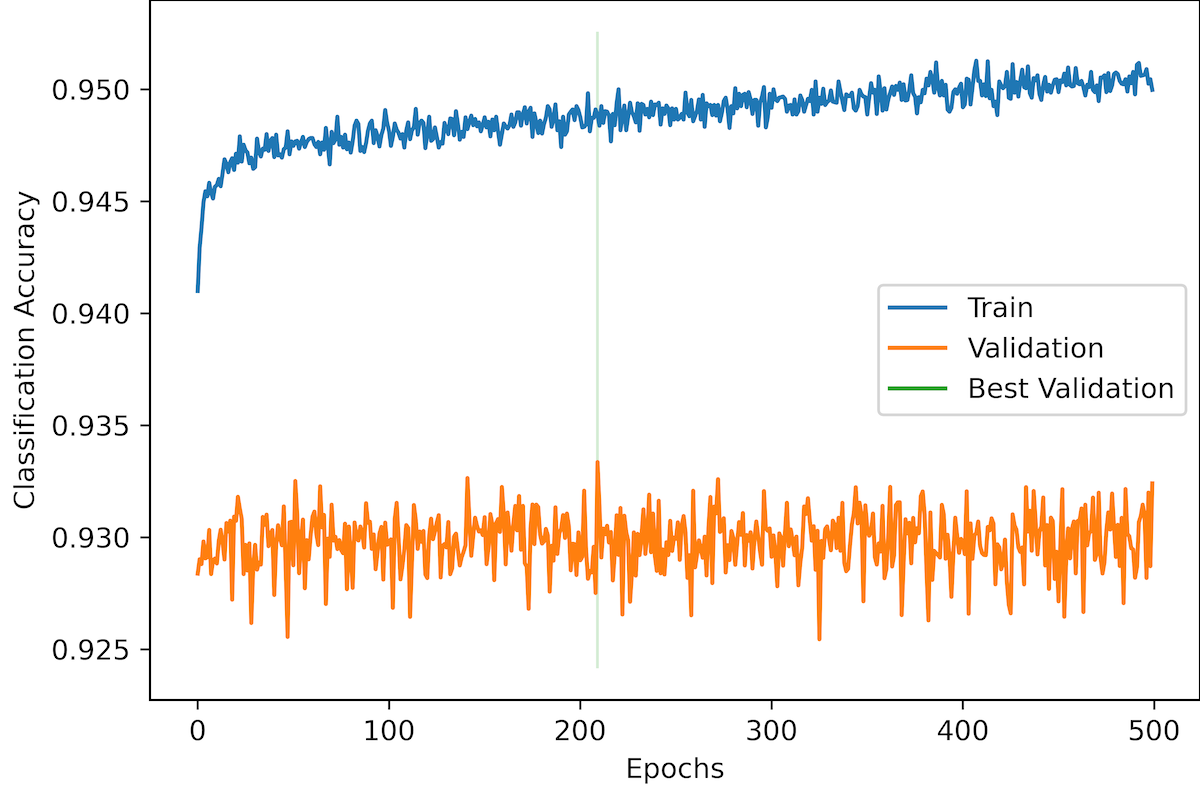
\includegraphics[width=0.45\textwidth]{src/cifar10_exp1_train1.png}}

\subfigure[CIFAR100]{
\label{Fig.sub.a1}
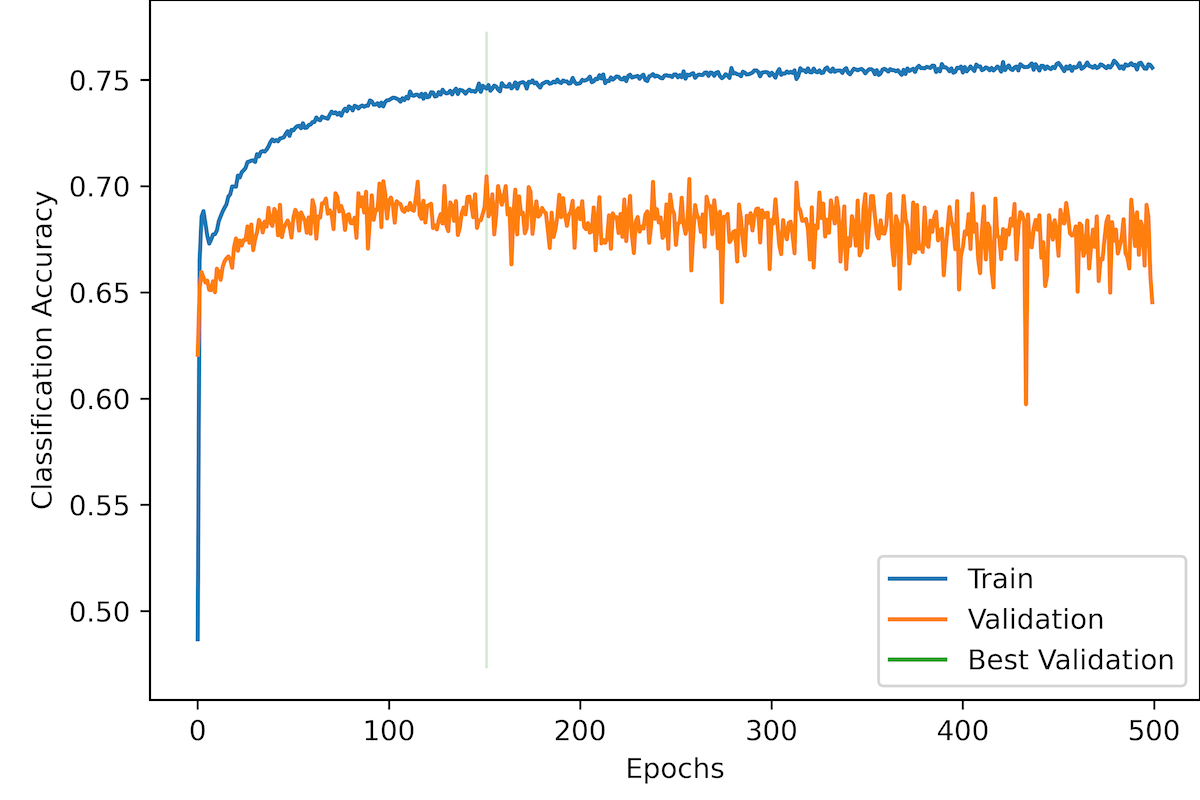
\includegraphics[width=0.45\textwidth]{src/cifar100_exp1_train.png}}
\subfigure[CIFAR100]{
\label{Fig.sub.a2}
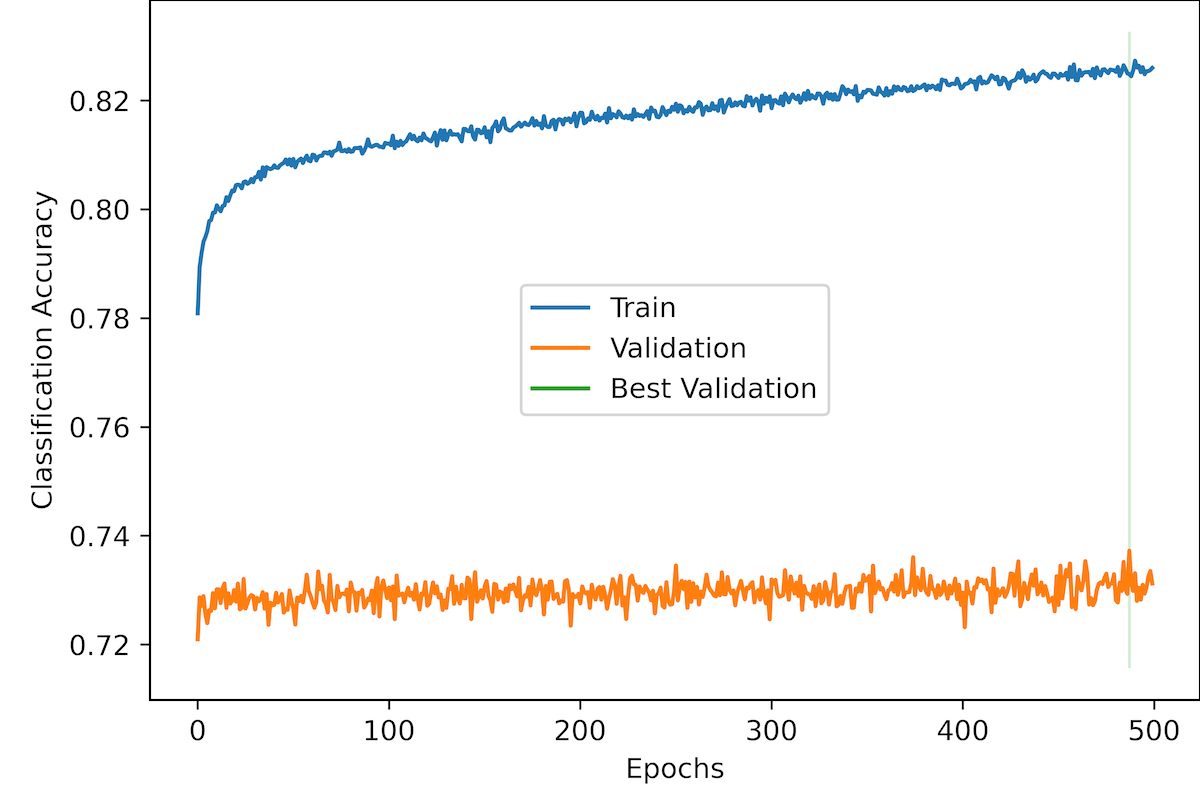
\includegraphics[width=0.45\textwidth]{src/cifar100_exp1_train1.png}}

\caption{The training history of CIFAR10 and CIFAR100. The left column is the first 500 epochs and the right column is the second 500 columns. The green line represents the best validation epoch.}
\label{Fig.extracthis}
\end{figure}

\begin{figure}[H]
\centering  
\subfigure[CIFAR10]{
\label{Fig.sub.a1}
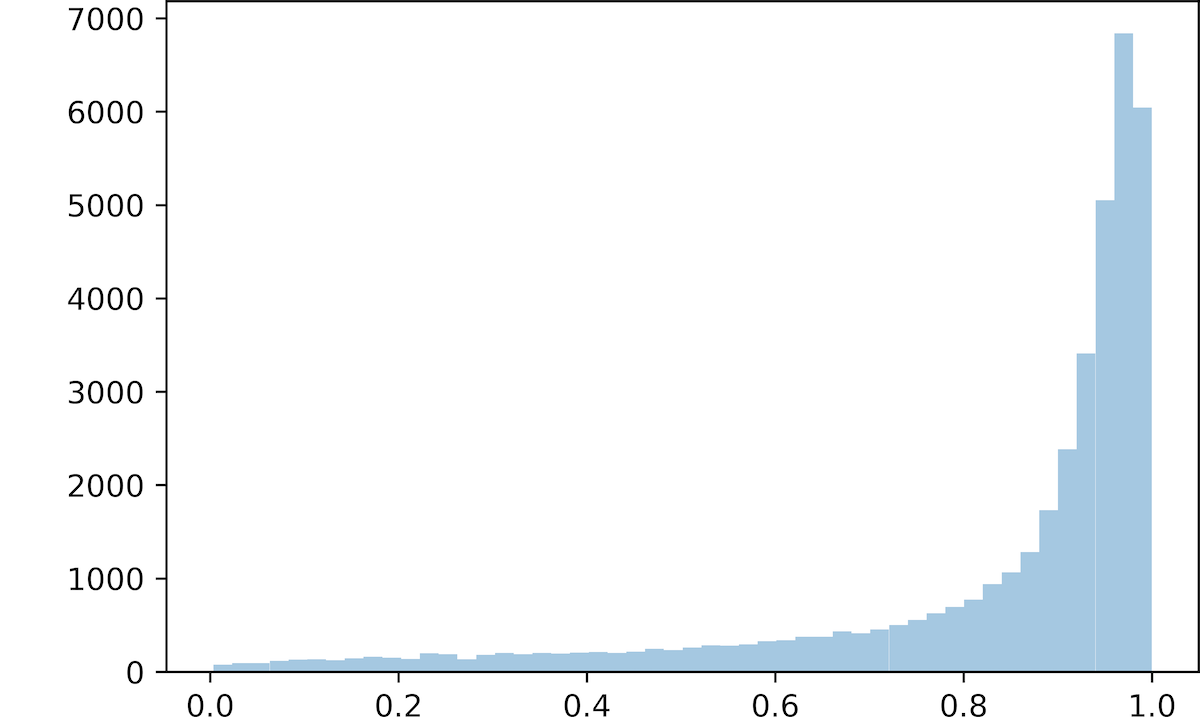
\includegraphics[width=0.45\textwidth]{src/cl_score_cifar10.png}}
\subfigure[CIFAR100]{
\label{Fig.sub.a2}
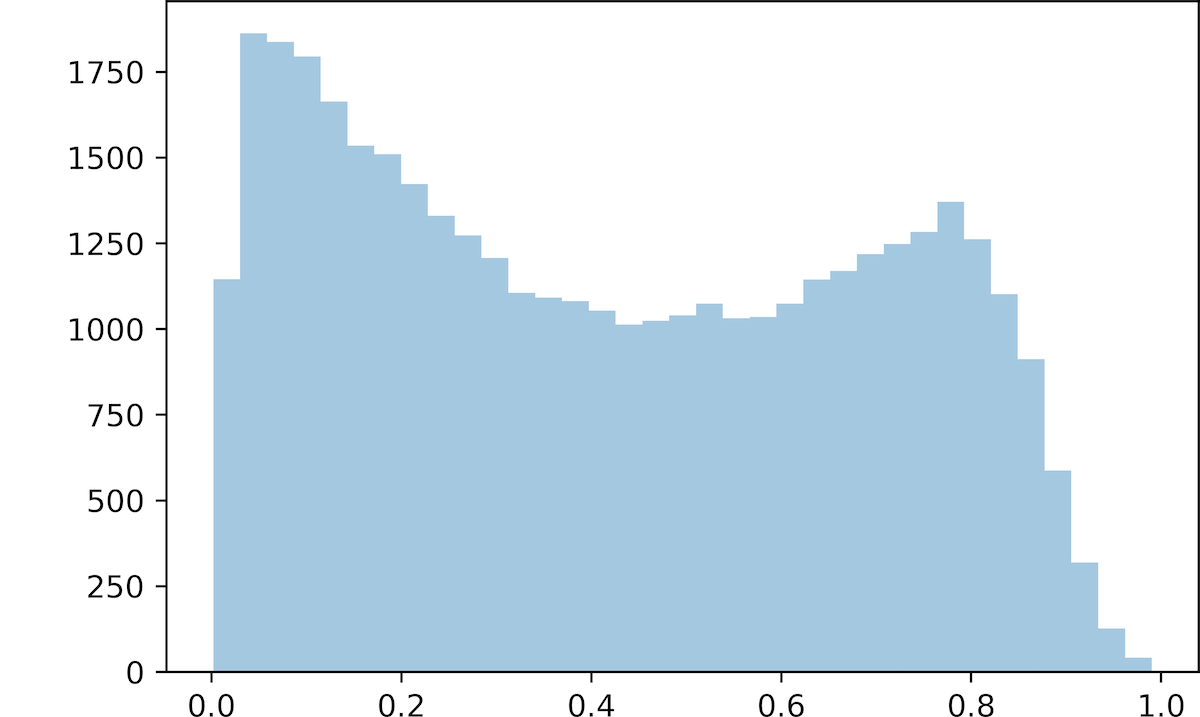
\includegraphics[width=0.45\textwidth]{src/cl_score_cifar100.png}}
\caption{Classification score distributions}
\label{Fig.clscores}
\end{figure}





\section{Experiment 2: Intrinsic Behaviour}
Obtaining the discriminative t-SNE plots, we assumed the FC layers to have learnt high quality compressed features. In this experiment, we tried to get an understanding of the intrinsic behaviours of these data reduction algorithms by visualising the selected CIFAR10 samples with red points. We managed to explain the behaviours with the answers to two questions: 
\begin{enumerate}
	\item What are the geometrical distributions of the selected samples?
	\item What are the classification score distributions of the selected samples?
\end{enumerate}

For each algorithm, the selection behaviours were further explored by tuning the hyper-parameters. We chose to use CIFAR10 for the reason that the quality of t-SNE projected blobs are more discriminative than CIFAR100 thus we can understand the behaviours easily. 

% POP
First of all, we present the POP selected  vsamples by adjusting the equal tolerance of the $resort\_by\_label$ function described in Algorithm \ref{pop_psudo}. For each  tolerance choice, we removed only pure inner samples whose weakness values are 128. Figure \ref{Fig.popcifar10} depicts that with proper threshold setting such as $et = 1$, we can select most samples along the blob contours as desired. Also, from Figure \ref{Fig.popcifar10.a1} and \ref{Fig.popcifar10.a2}, we observe a trend to select samples closer to the boundary between two adjacent blobs rather than cover the whole contours. This behaviour can guide linear classifiers to build the proper decision boundaries. Another advantage of POP is the fast compute speed. It took us 33.27 seconds on average to get the result. However, POP was designed to process integer features. It is difficult to choose the suitable tolerance value and keep just enough samples. Our experiments indicate that the number of samples far from the boundary decreases much faster than expected by increasing the tolerance value. One possible reason is that we normalised the compressed features so the value range is too compact. This makes POP hard to use for image datasets. 
   
\begin{figure}
\centering  
\subfigure{
\label{Fig.popcifar10.a1}
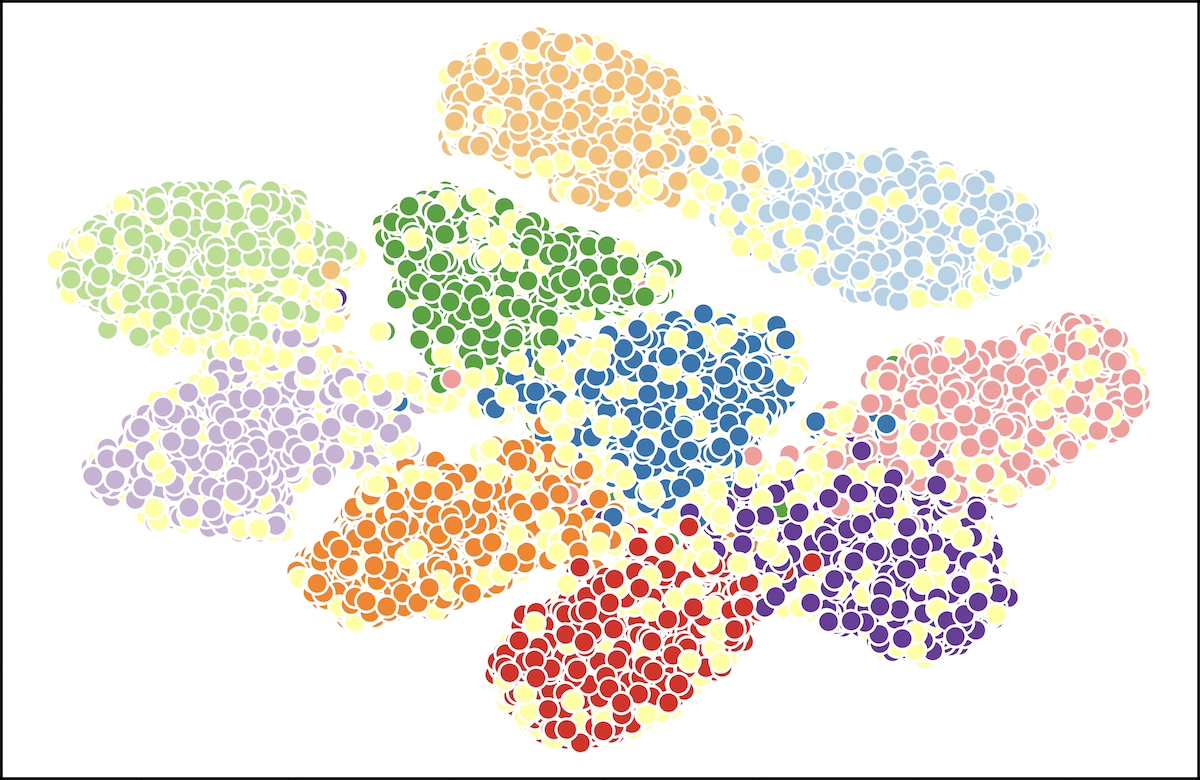
\includegraphics[width=0.32\textwidth]{src/pop-cifar10-1.png}}
\subfigure{
\label{Fig.popcifar10.a2}
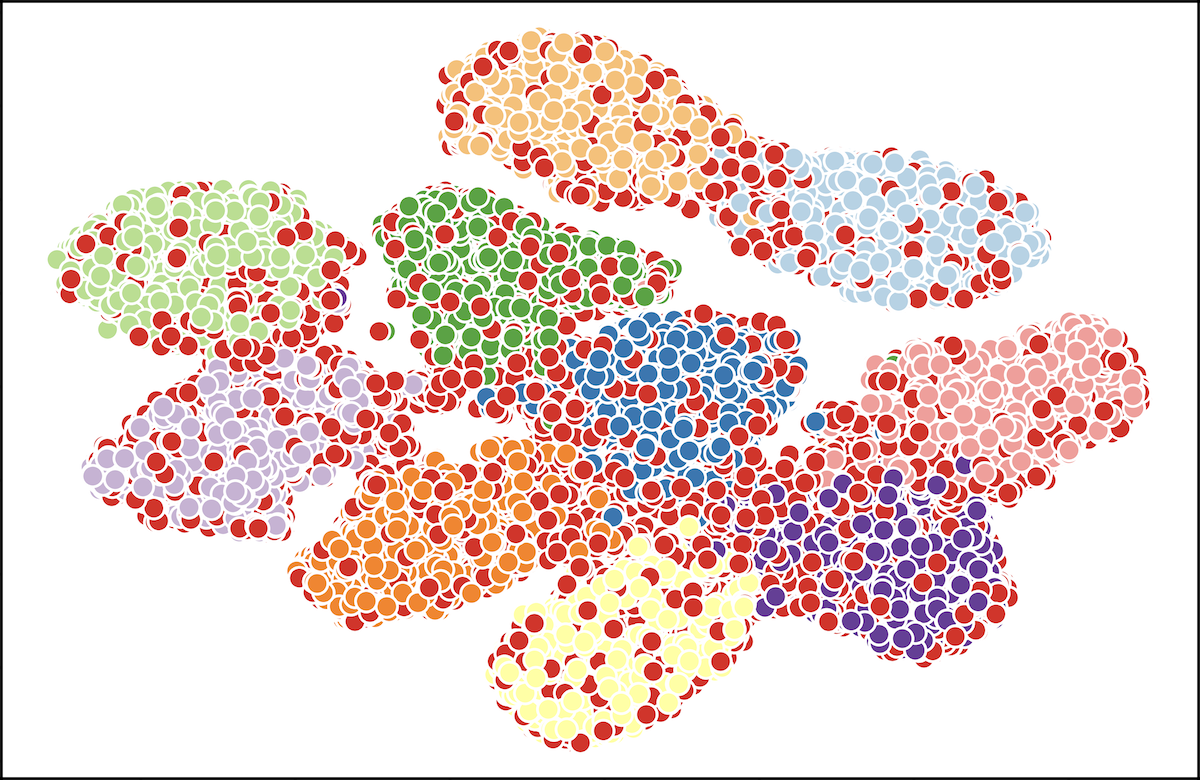
\includegraphics[width=0.32\textwidth]{src/pop-cifar10-5.png}}
\subfigure{
\label{Fig.sub.a1}
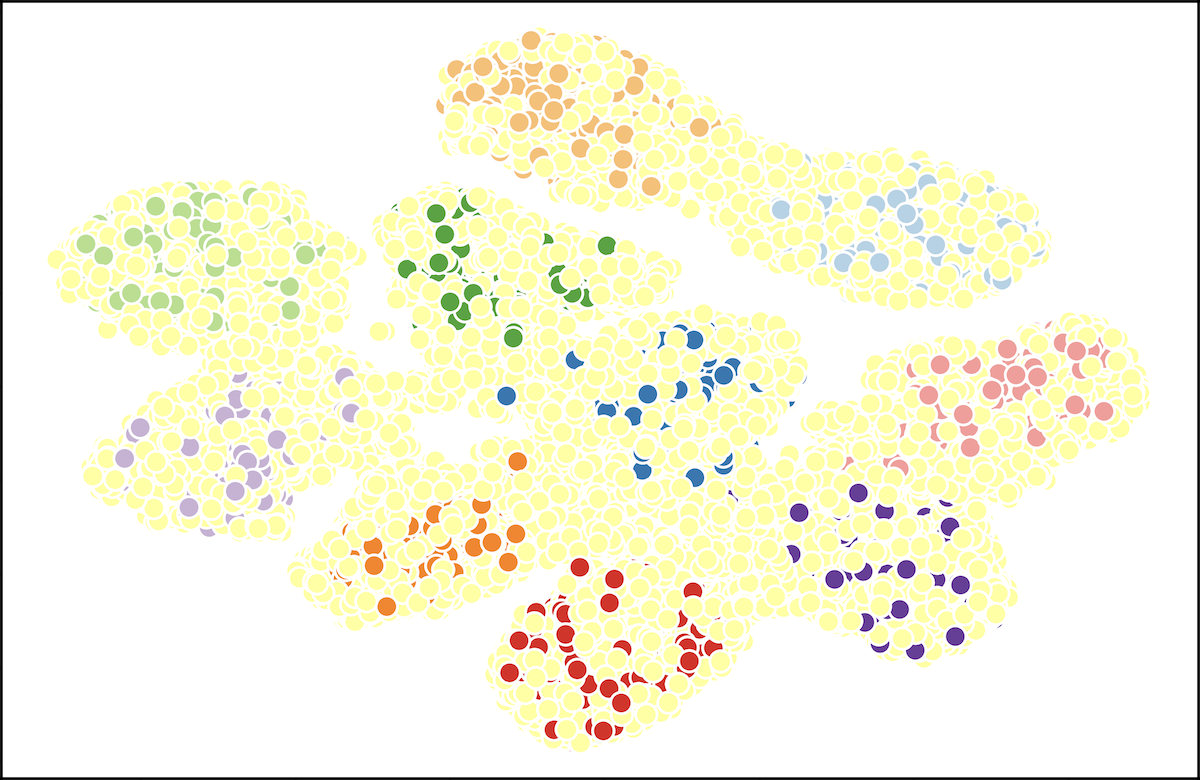
\includegraphics[width=0.32\textwidth]{src/pop-cifar10-01.png}}

\setcounter{subfigure}{0}
\subfigure[T=1, 8701 samples, 33.3s]{
\label{Fig.popcifar10.a1}
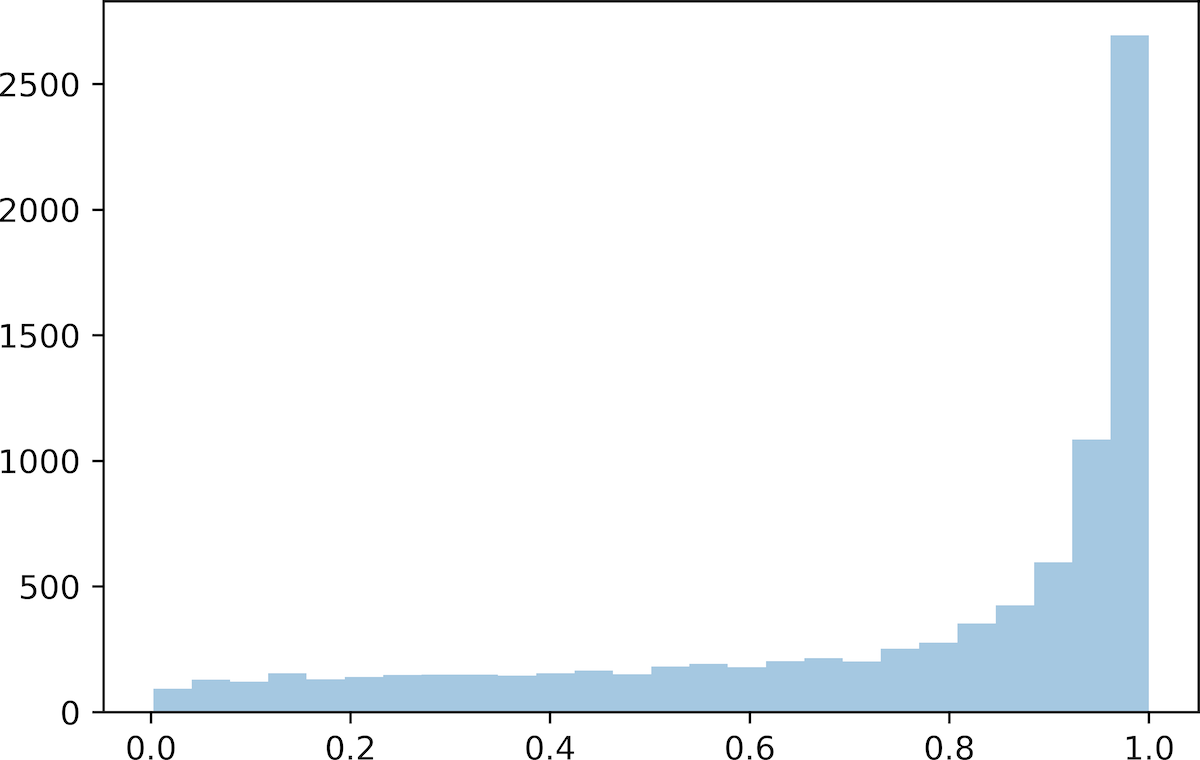
\includegraphics[width=0.32\textwidth]{src/pop-cifar10-dis-1.png}}
\subfigure[T=0.5, 14111 samples, 29.7s]{
\label{Fig.popcifar10.a2}
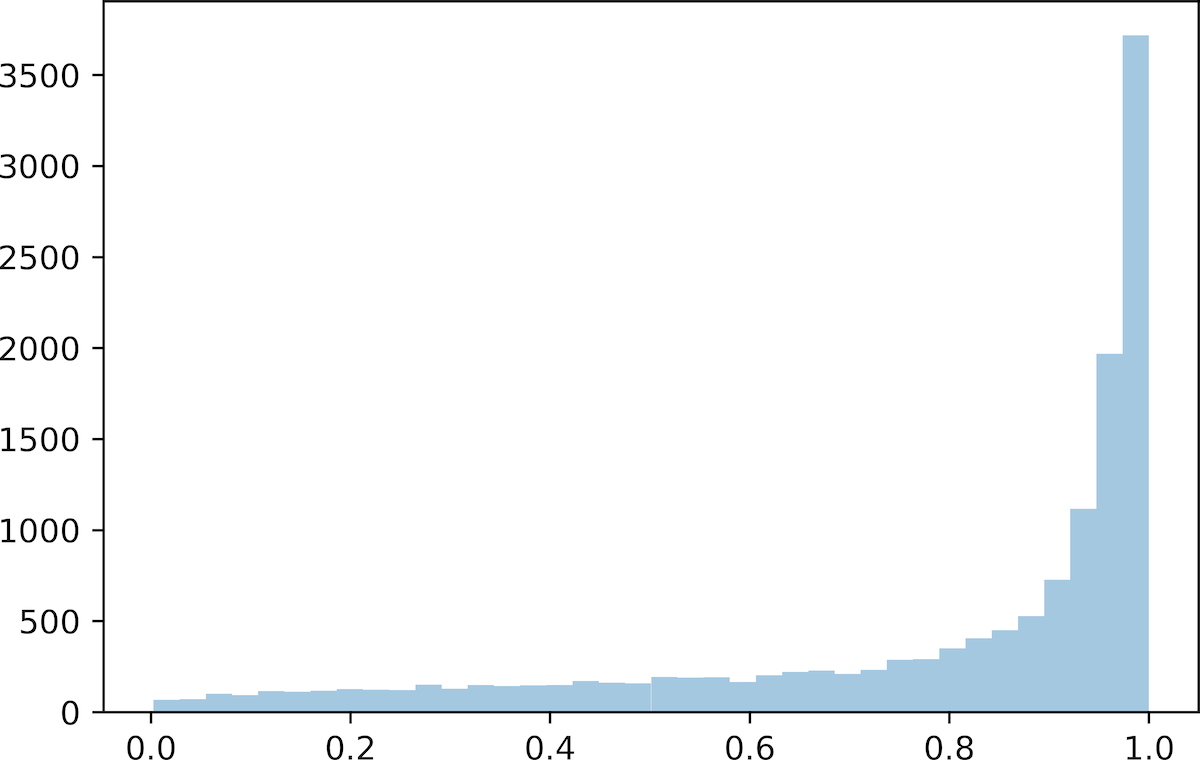
\includegraphics[width=0.32\textwidth]{src/pop-cifar10-dis-05.png}}
\subfigure[T=0.1, 31966 samples, 36.8s]{
\label{Fig.popcifar10.a3}
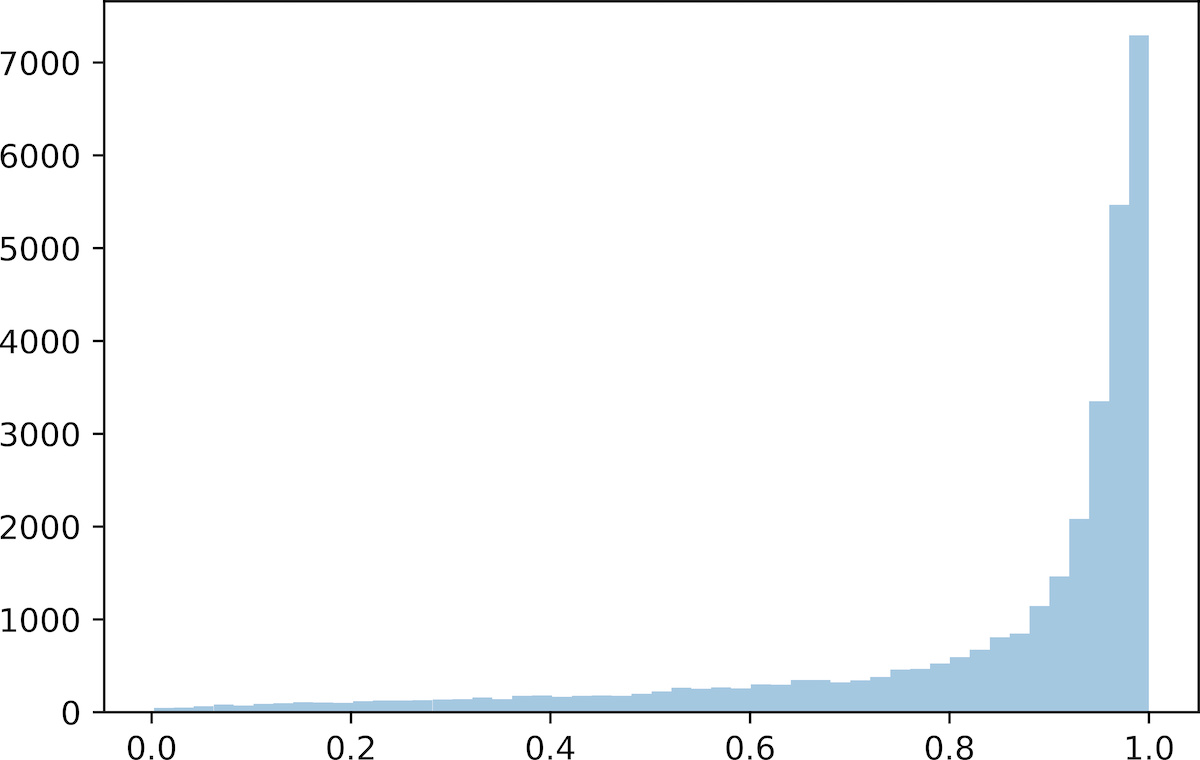
\includegraphics[width=0.32\textwidth]{src/pop-cifar10-dis-01.png}}
\caption{POP tune threshold}
\label{Fig.popcifar10}
\end{figure}

The second algorithm we explored is EGDIS by tuning the hyper-parameter $k$ of the $knn$ classifier. Figure \ref{Fig.egdiscifar10} presents how the selection pattern varies with $k$ values 3, 5, and 7. Our first discovery is that EGDIS tends to select all misclassified samples together with samples surrounding them. Compared with Figure \ref{Fig.tsne2}, only a few samples still exist with different colours. Also, by increasing the value of $k$, fewer inner samples and boundary are selected. To explain these results, we need to know how EGDIS works with hyper-parameter $k$. In short, higher $k$ values require boundary samples to have more neighbours from different classes. Based on this mechanism, we can infer that most misplaced samples are alone and surrounded by correctly classified samples. For these isolated samples, they would be considered as boundary samples and have enough number of neighbours to be selected. For samples near the boundary, fewer samples will be qualified and only those closely contacted with other blobs would be selected. For dense samples near isolated misplaced points, some of them may be categorised as boundary samples and wouldn't be selected anymore.


\begin{figure}[H]
\centering  
\subfigure{
\label{Fig.sub.a1}
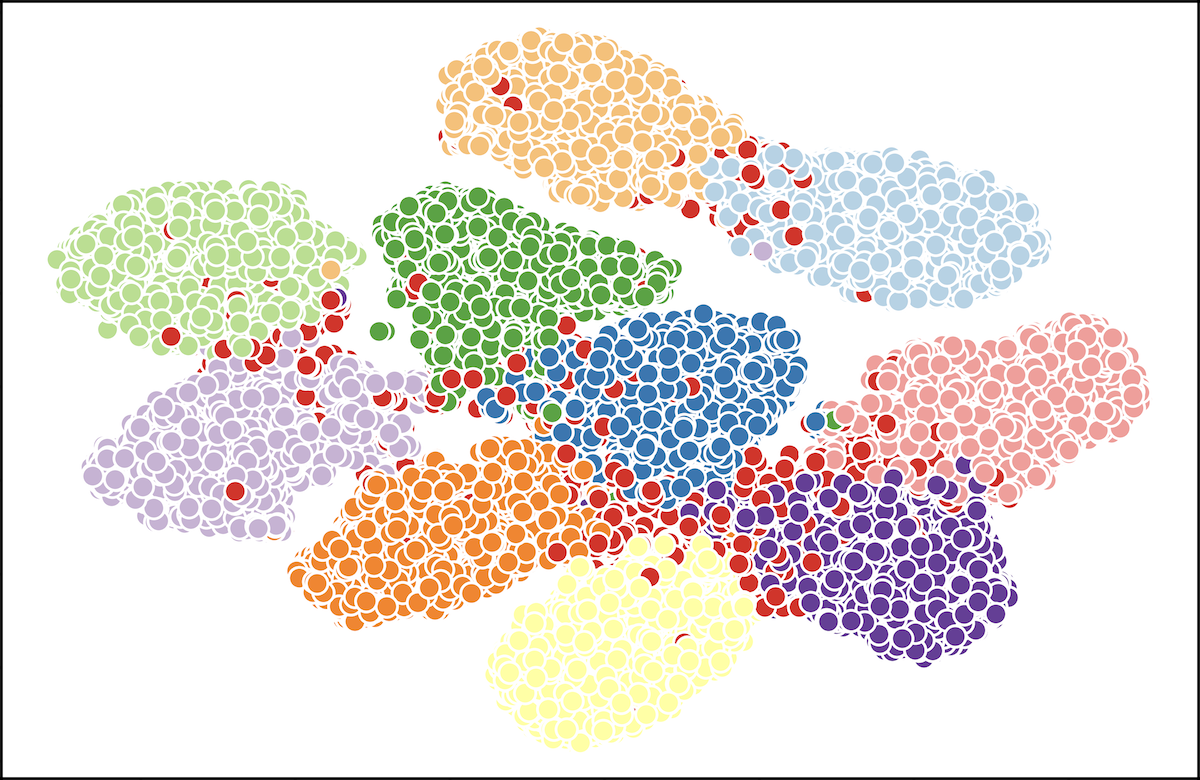
\includegraphics[width=0.32\textwidth]{src/egdis-cifar10-8.png}}
\subfigure{
\label{Fig.sub.a2}
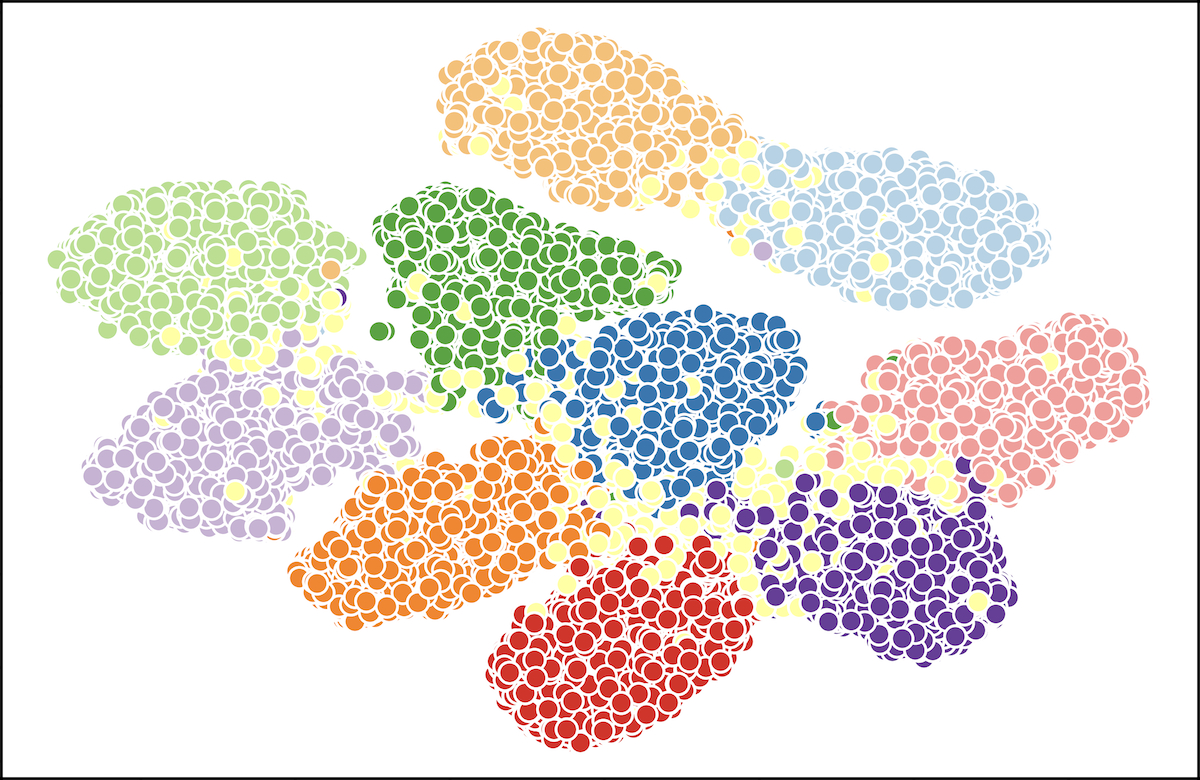
\includegraphics[width=0.32\textwidth]{src/egdis-cifar10-6.png}}
\subfigure{
\label{Fig.sub.a1}
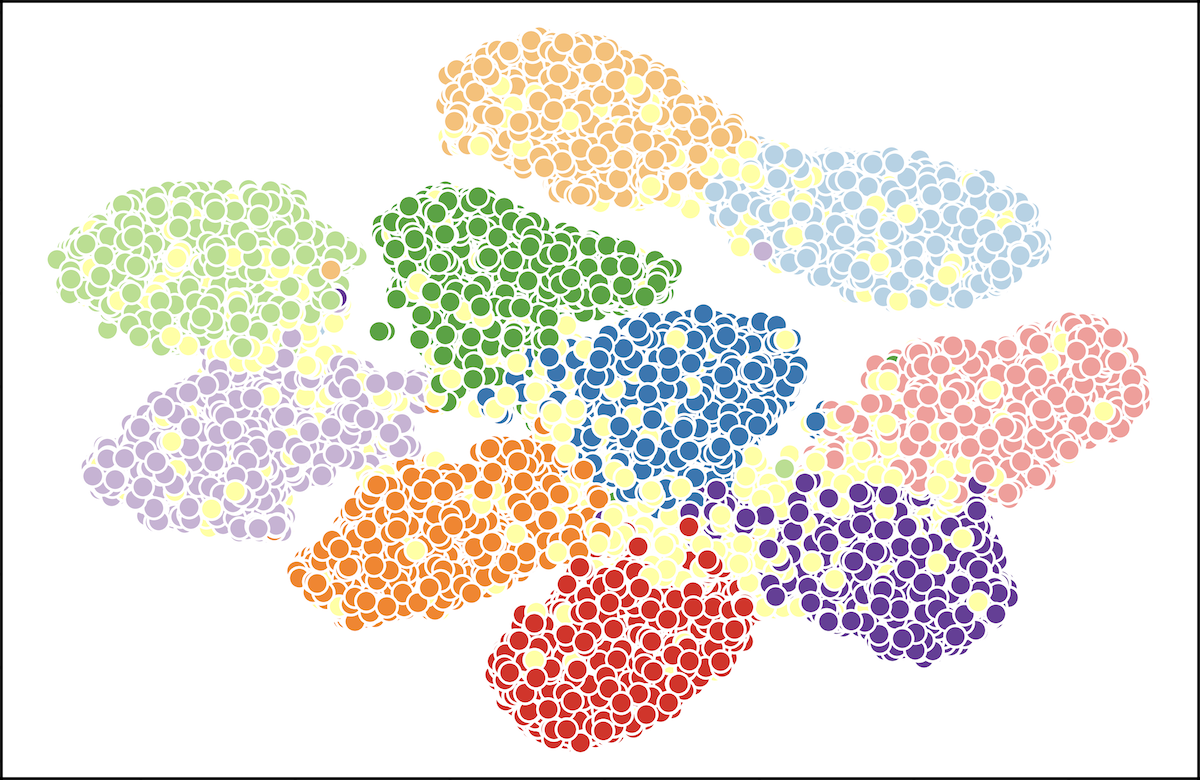
\includegraphics[width=0.32\textwidth]{src/egdis-cifar10-4.png}}

\setcounter{subfigure}{0}
\subfigure[k=7, 2799 samples, 14min 27s]{
\label{Fig.egdiscifar10x.a1}
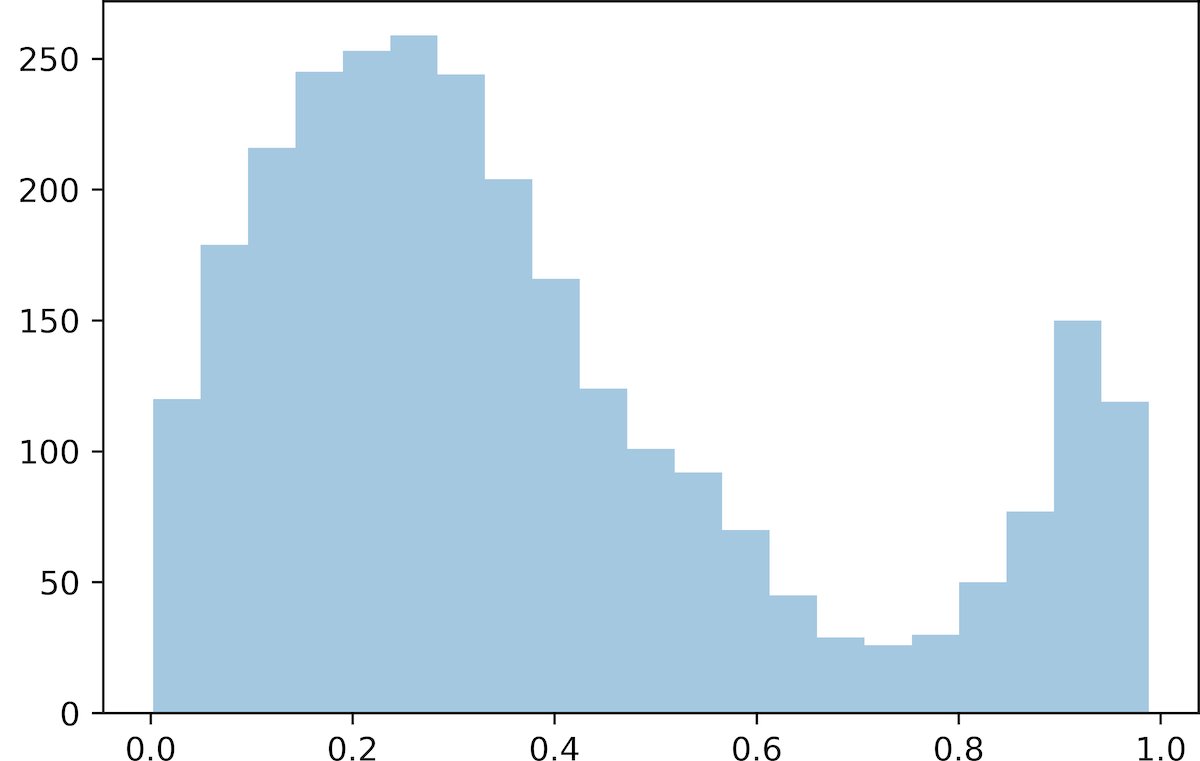
\includegraphics[width=0.32\textwidth]{src/egdis-cifar10-dis-7.png}}
\subfigure[k=5, 3483 samples, 15min 7s]{
\label{Fig.egdiscifar10.a2}
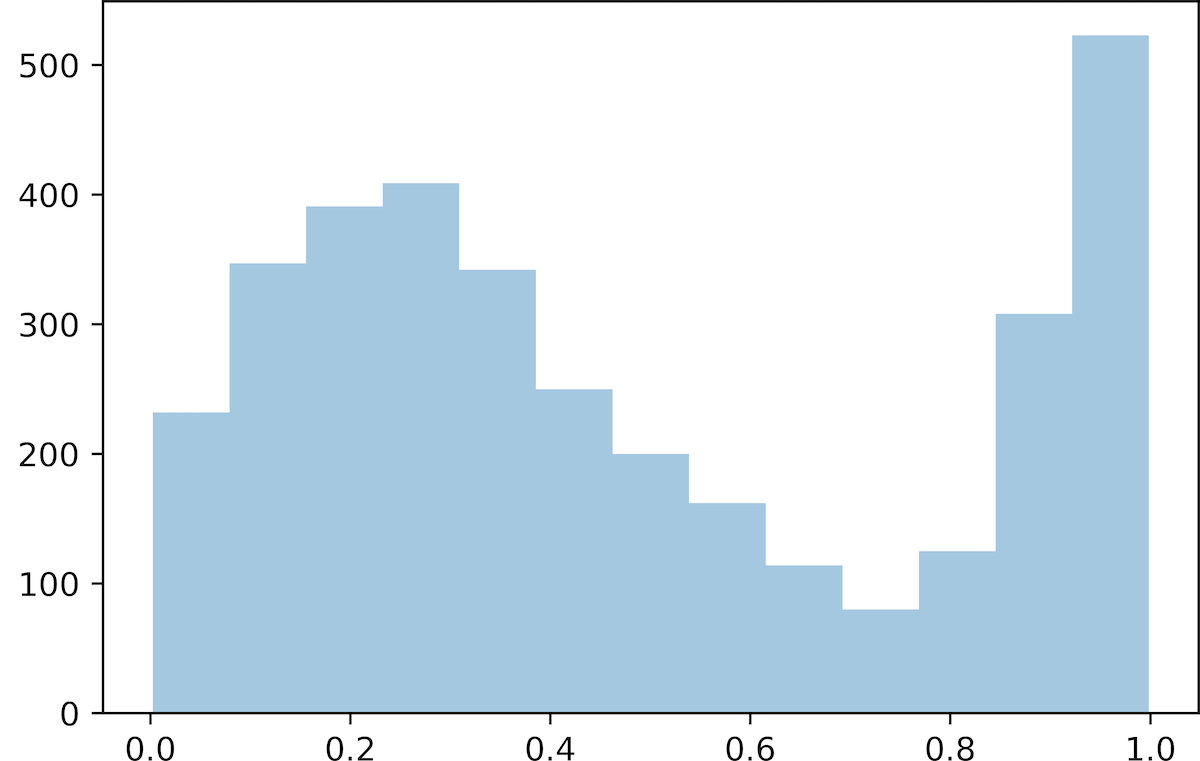
\includegraphics[width=0.32\textwidth]{src/egdis-cifar10-dis-5.png}}
\subfigure[k=3, 5966 samples, 14min 56s]{
\label{Fig.egdiscifar10.a3}
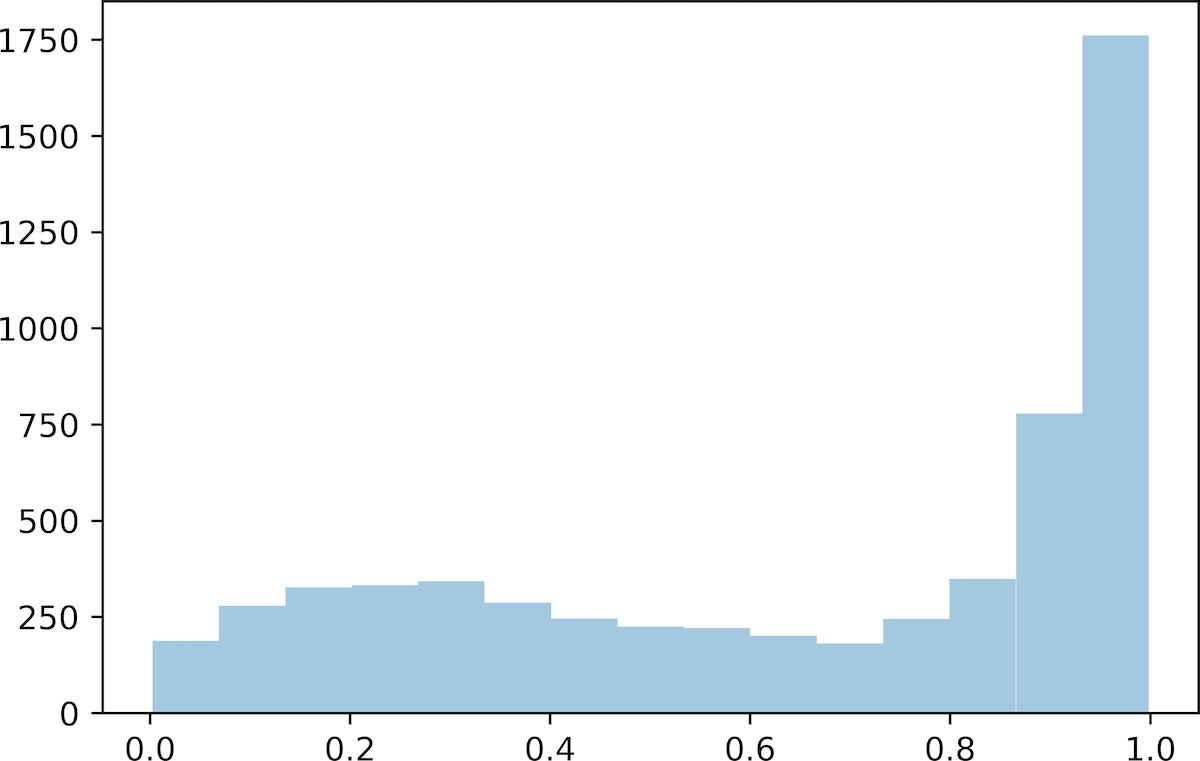
\includegraphics[width=0.32\textwidth]{src/egdis-cifar10-dis-3.png}}
\caption{EGDIS tune kNN}
\label{Fig.egdiscifar10}
\end{figure}

The drawback of EGDIS is the global density calculation which computes the distance between all training samples. In our experiments, it took us on average 14 minutes 50 seconds to get all the selected samples and we only need about 12 seconds to select the boundary samples. Figure \ref{Fig.egdisboscores} shows the score distribution of EDGIS selected boundary samples with $k=3$. Compared with the second column of Figure \ref{Fig.egdiscifar10.a3}, the main difference is the lack of high score samples. Therefore, if we choose to select higher score samples from the score list, we can combine them with EGDIS selected boundary samples and get a similar EGDIS score distribution within about 20 seconds. We will mention this topic in the next few paragraphs.

\begin{figure}[H]
\centering  
\subfigure[Scores]{
\label{Fig.sub.a1}
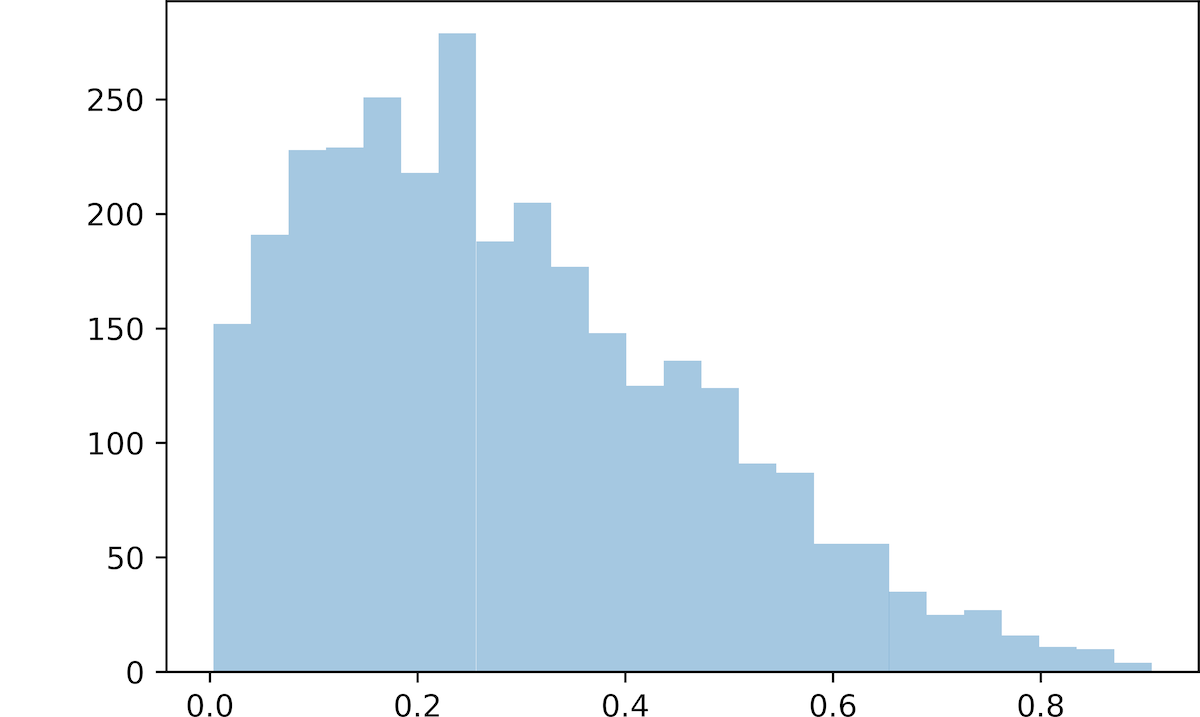
\includegraphics[width=0.45\textwidth]{src/boundarydis-cifar10-dis.png}}
\subfigure[Plots]{
\label{Fig.sub.a2}
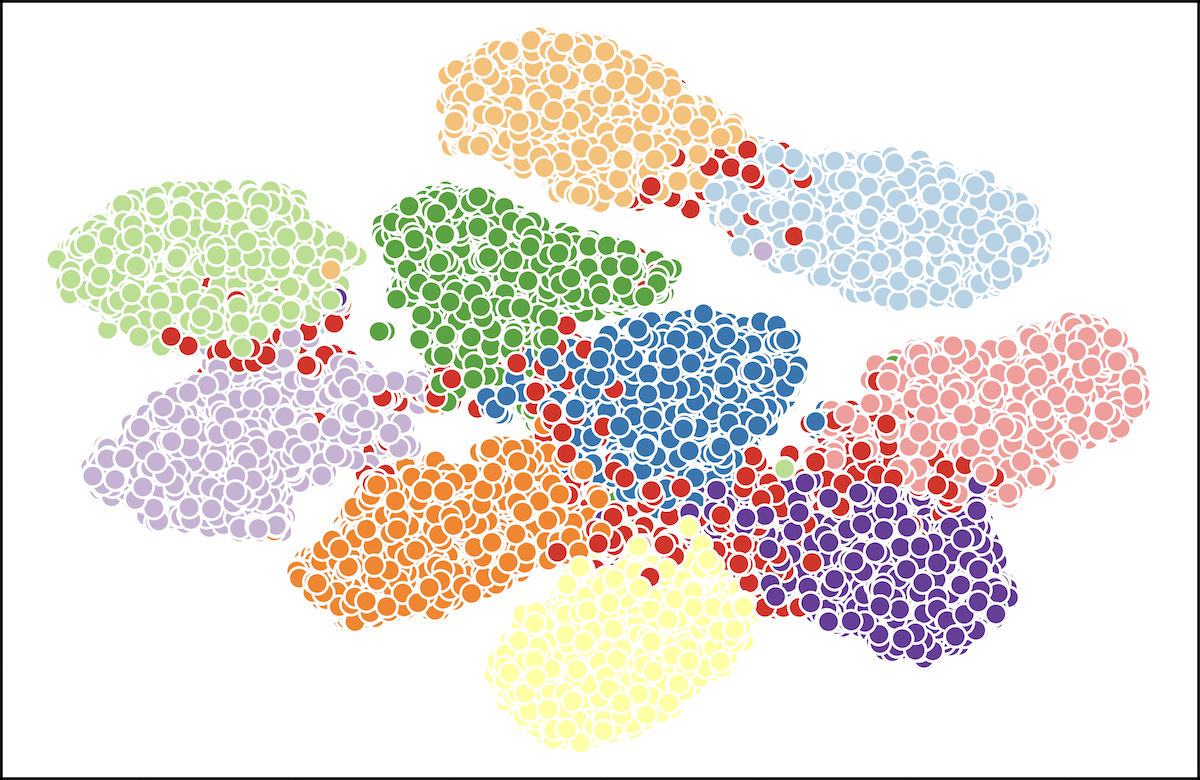
\includegraphics[width=0.45\textwidth]{src/egdis-boundary-cifar10.png}}
\caption{EGDIS boundary score distribution}
\label{Fig.egdisboscores}
\end{figure}

Next, we visualised the selection preference of CL in Figure \ref{Fig.clcifar10}. We selected different percentages of samples and the selection pattern is very obvious. We can see that CL tends to select only high score samples, and these samples are lying in the opposite direction as the EGDIS boundary samples. This is what we expected because samples far from the decision boundary would have high scores if the classifier.  From the score distributions, we can see that all selected samples are easy to classify for deep learning. This reminds us to combine these high score samples with EGDIS boundary samples. We can construct a limit of the blobs. However, the downside is that no inner samples are selected and the limit borders are not complete. We can not capture the whole shape of the blobs and the results are more like two isolated blobs for each class. With linear regression model, the boundary cannot be recovered precisely thus we may get lower accuracy.

\begin{figure}[H]
\centering  
\subfigure{
\label{Fig.sub.a1}
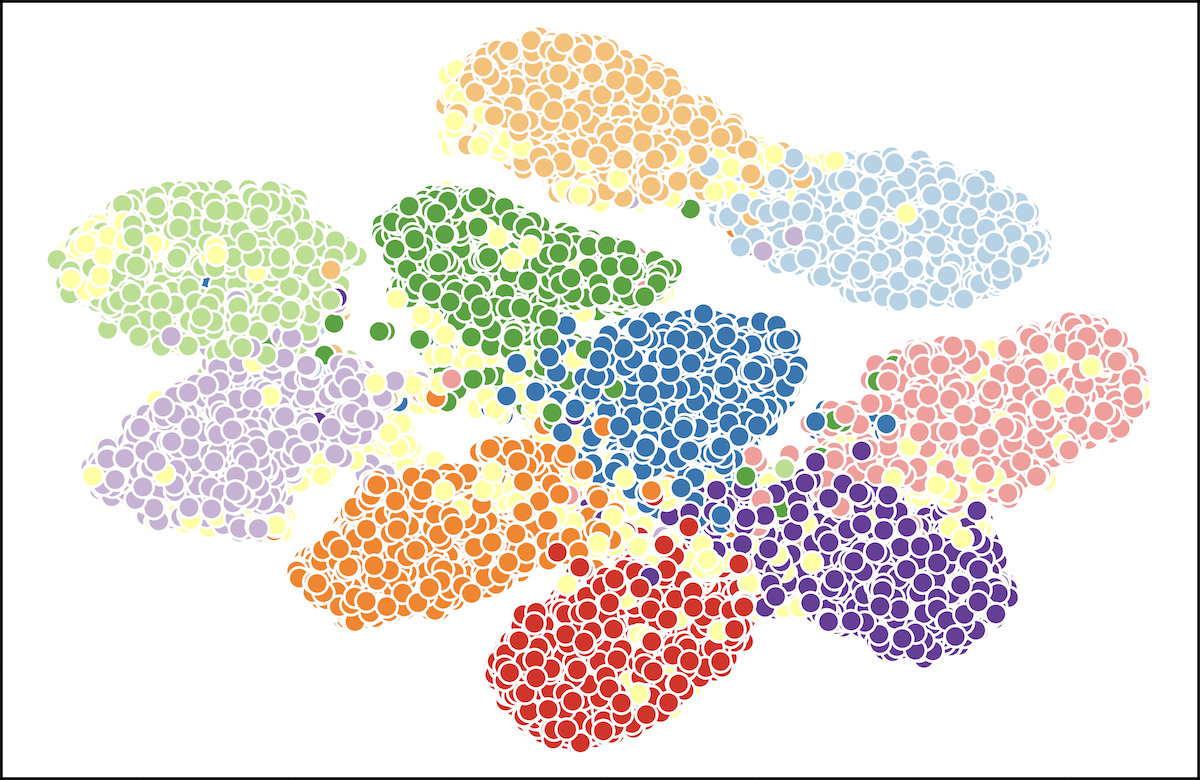
\includegraphics[width=0.32\textwidth]{src/cl-cifar10-1.png}}
\subfigure{
\label{Fig.sub.a2}
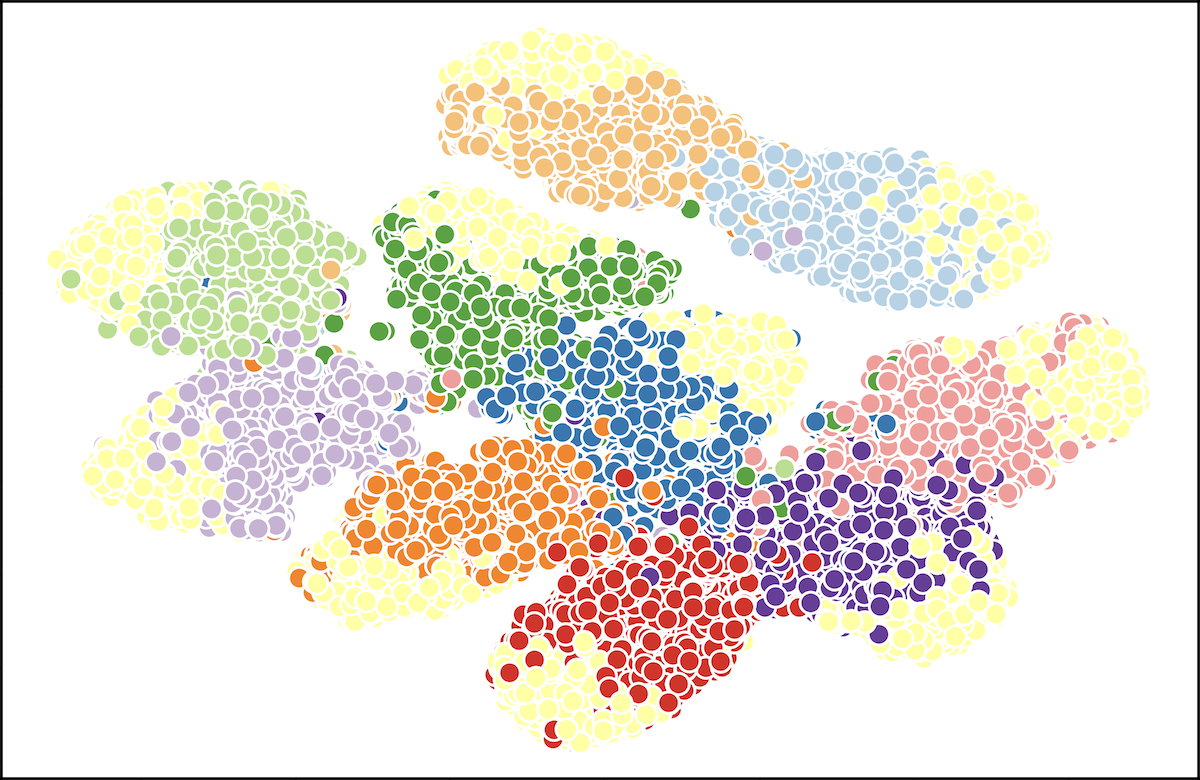
\includegraphics[width=0.32\textwidth]{src/cl-cifar10-3.png}}
\subfigure{
\label{Fig.sub.a1}
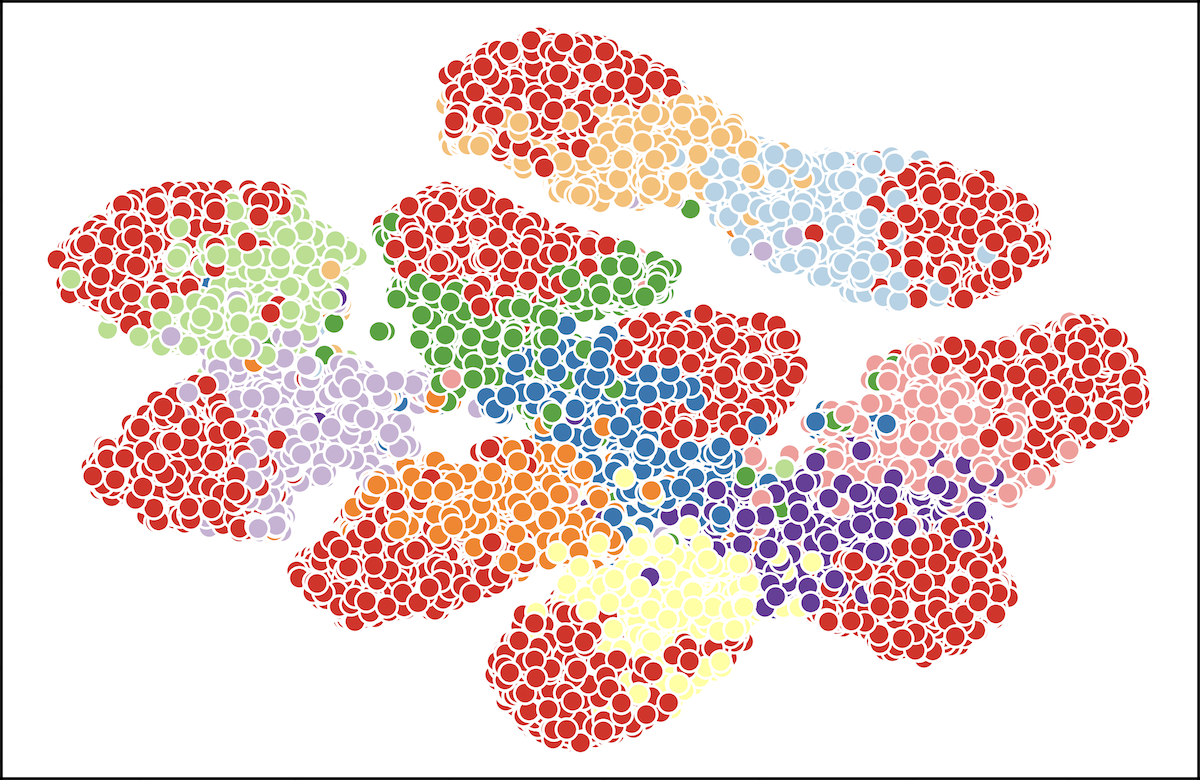
\includegraphics[width=0.32\textwidth]{src/cl-cifar10-5.png}}

\setcounter{subfigure}{0}
\subfigure[P=10\%, 4000 samples]{
\label{Fig.sub.a1}
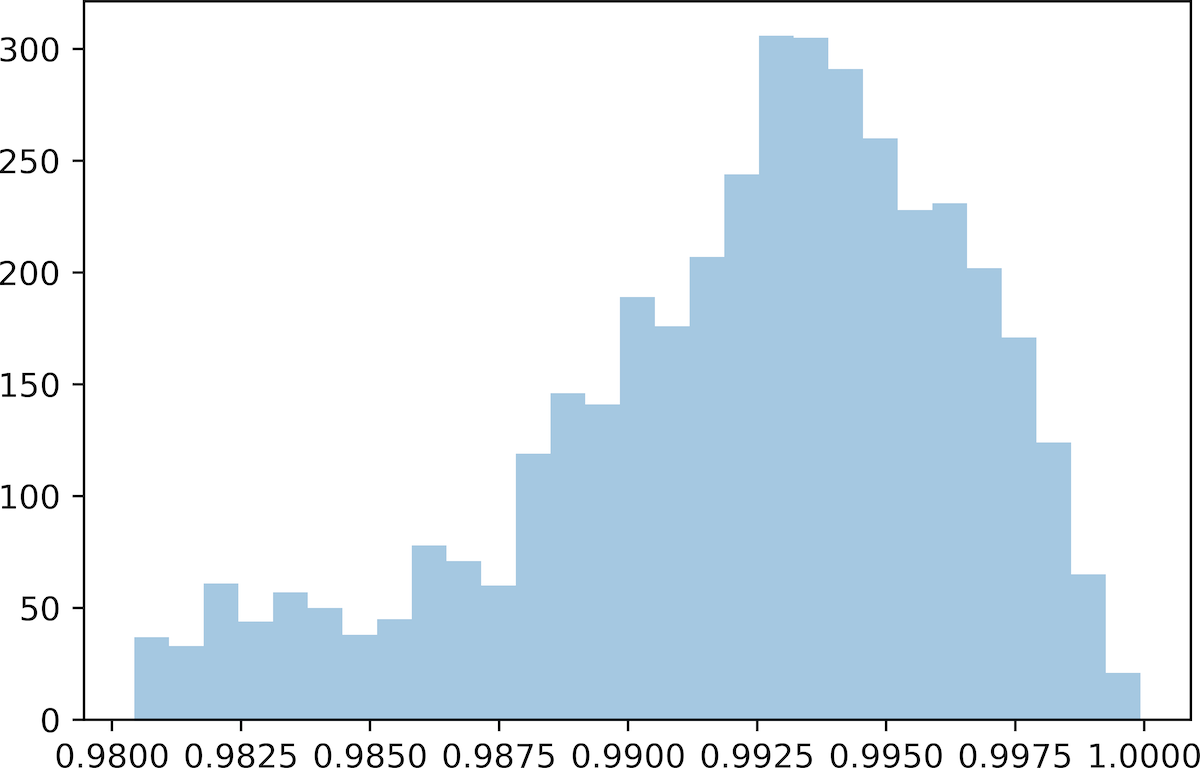
\includegraphics[width=0.32\textwidth]{src/cl-cifar10-1-scoredis.png}}
\subfigure[P=30\%, 12000 samples]{
\label{Fig.sub.a2}
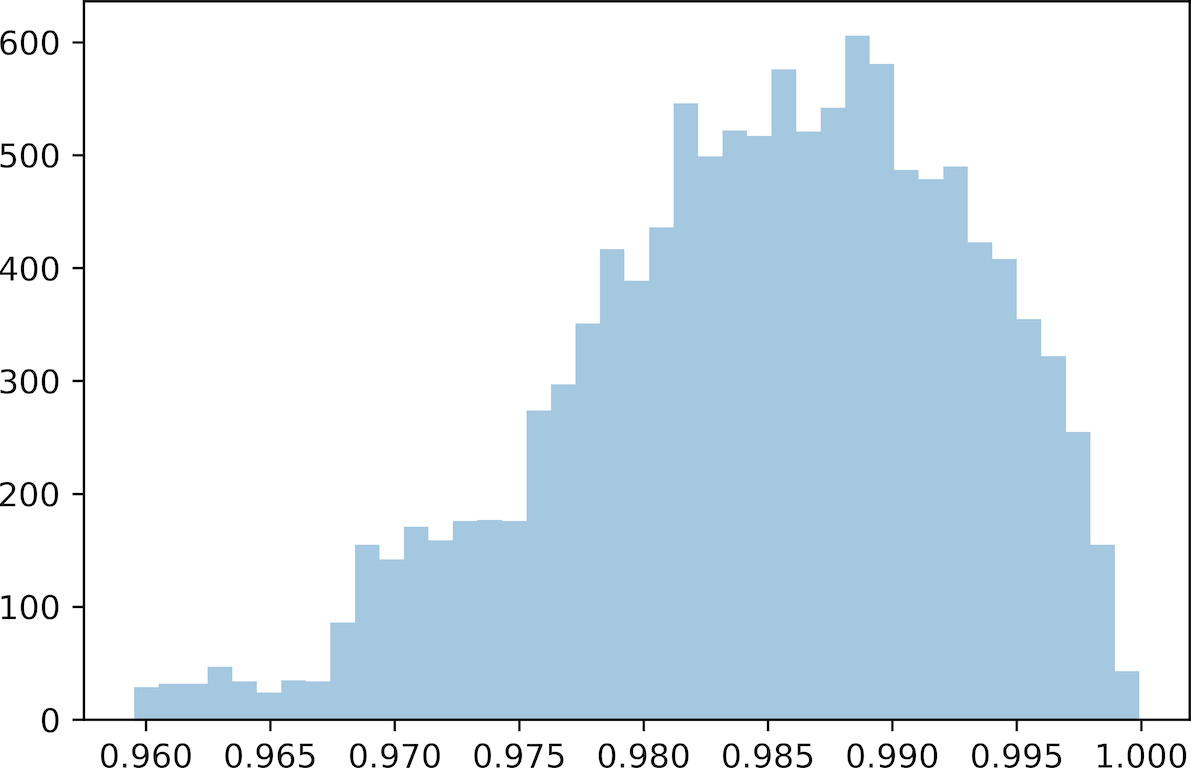
\includegraphics[width=0.32\textwidth]{src/cl-cifar10-3-scoredis.png}}
\subfigure[P=50\%, 20000 samples]{
\label{Fig.sub.a1}
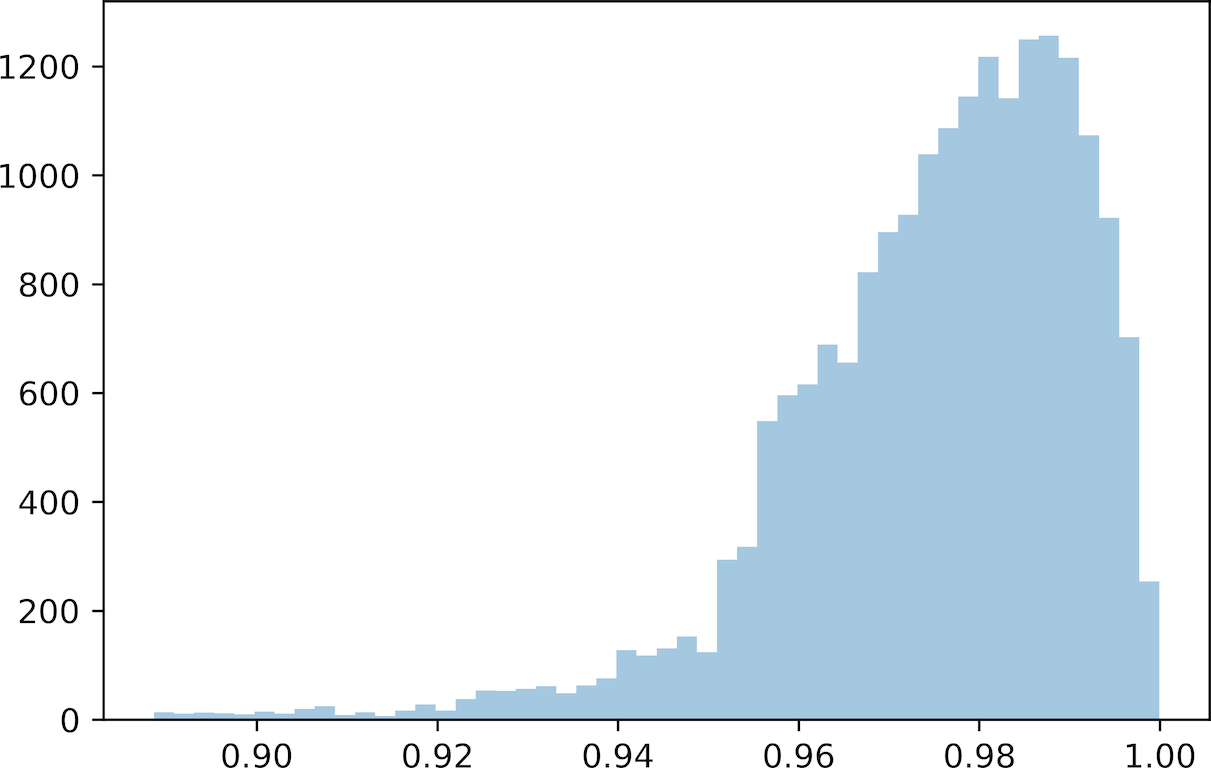
\includegraphics[width=0.32\textwidth]{src/cl-cifar10-5-scoredis.png}}
\caption{CL tune selection percentage}
\label{Fig.clcifar10}
\end{figure}

Rather than selecting only the top score samples, we proposed WCL to randomly select samples within each class based on the sample score. The results are shown in the first column of Figure \ref{Fig.wclcifar10}. Although most samples are selected from the high score region, there are some sample selected from the lower score regions. The problem is that less samples near the EGDIS boundary are selected. The boundary between close blobs are blurry thus we cannot guarantee the performance.



\begin{figure}[H]
\centering  
\subfigure{
\label{Fig.sub.a1}
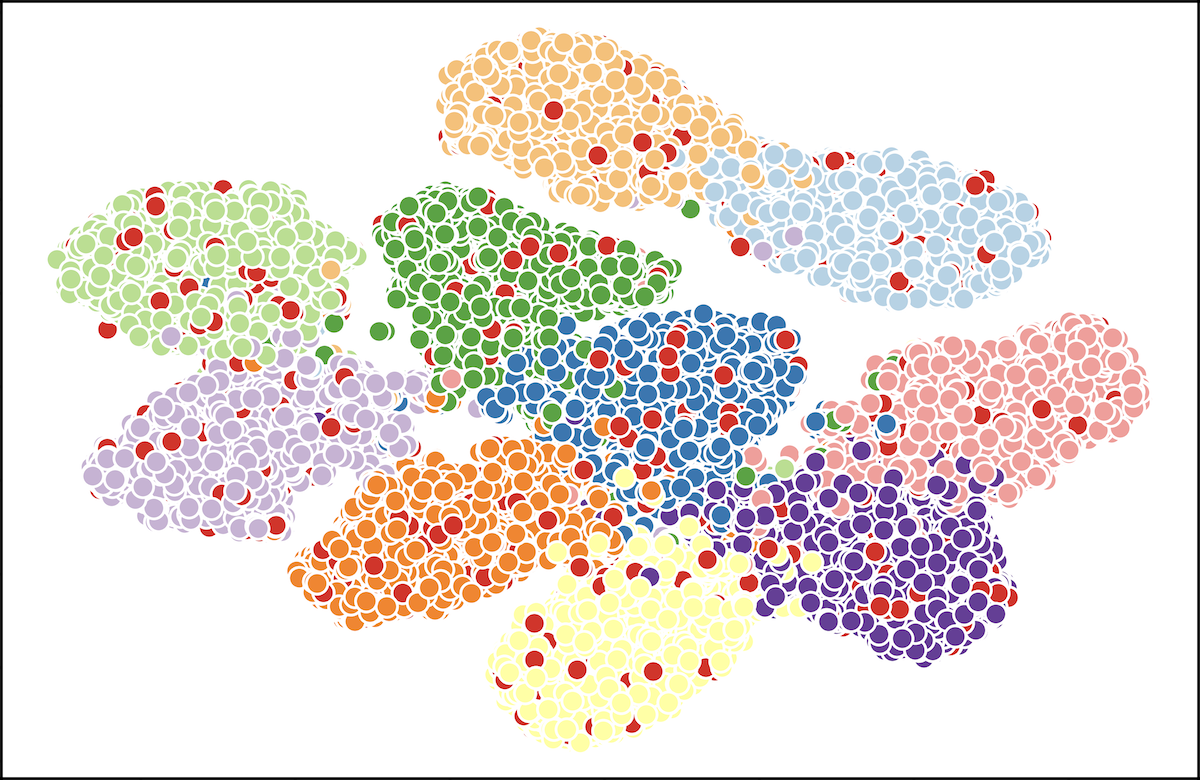
\includegraphics[width=0.32\textwidth]{src/wcl-cifar10-1.png}}
\subfigure{
\label{Fig.sub.a2}
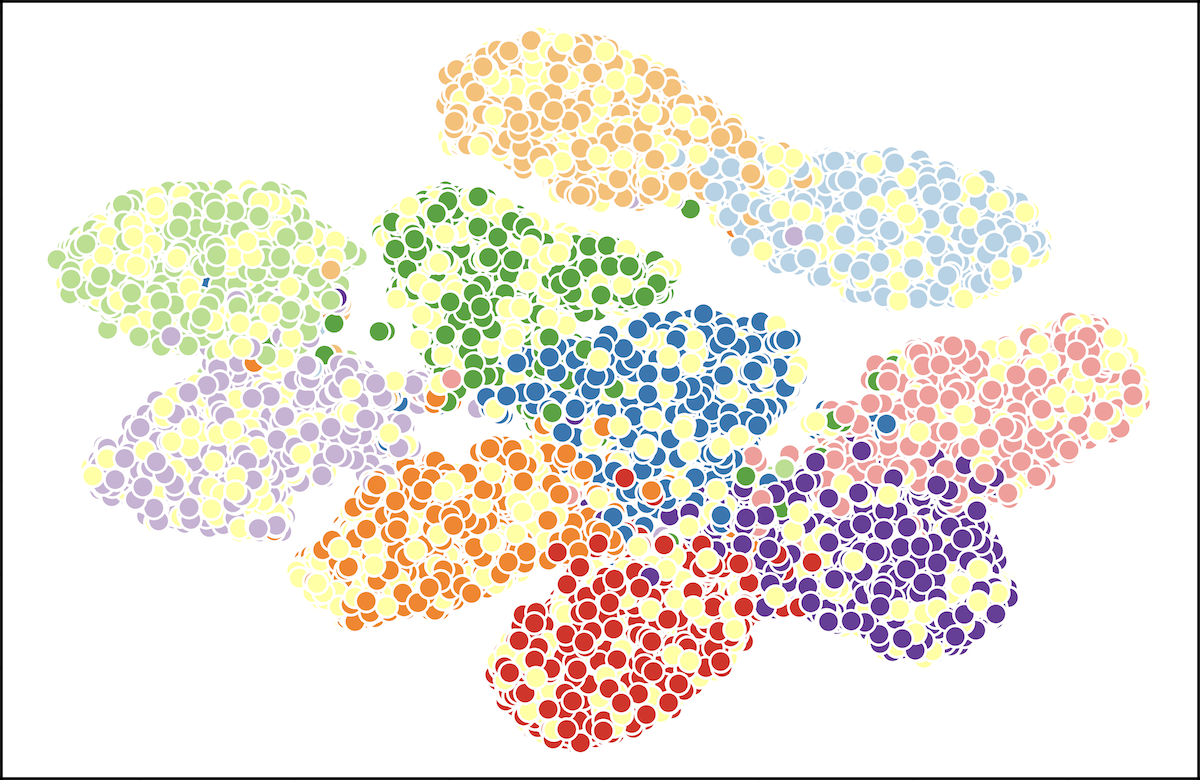
\includegraphics[width=0.32\textwidth]{src/wcl-cifar10-3.png}}
\subfigure{
\label{Fig.sub.a1}
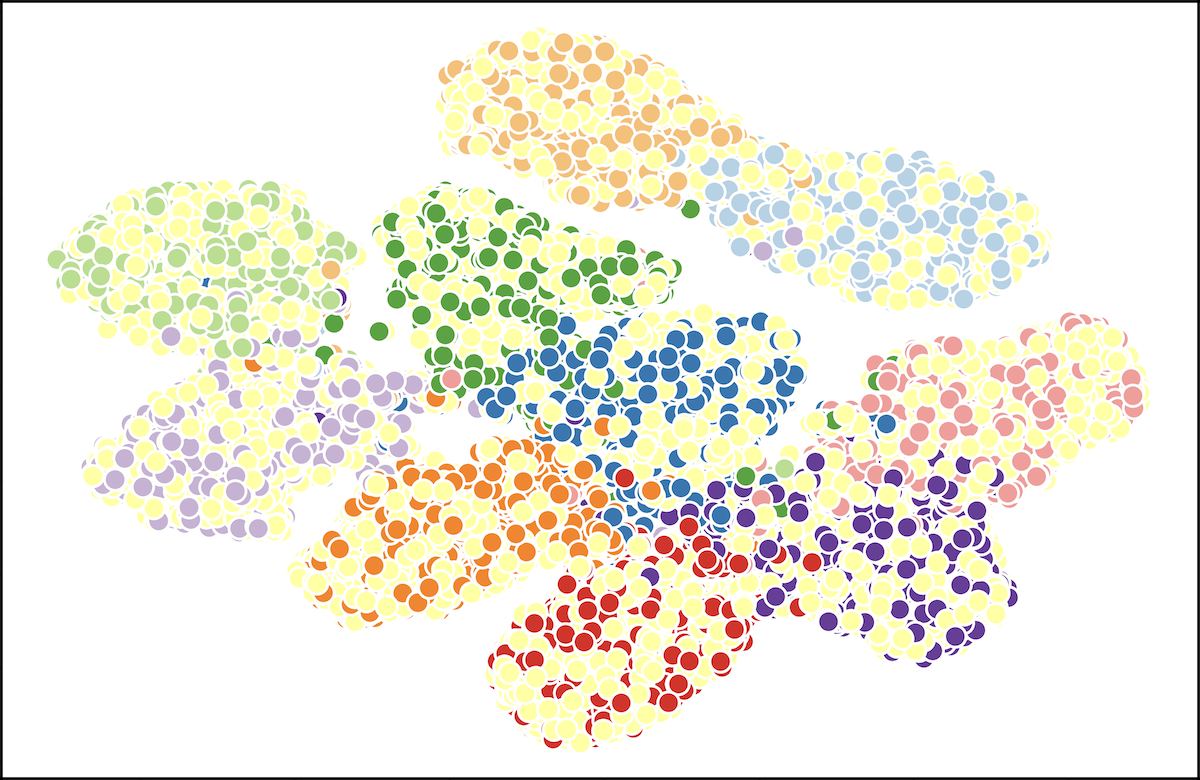
\includegraphics[width=0.32\textwidth]{src/wcl-cifar10-5.png}}

\setcounter{subfigure}{0}
\subfigure[P=10\%, 4000 samples]{
\label{Fig.sub.a1}
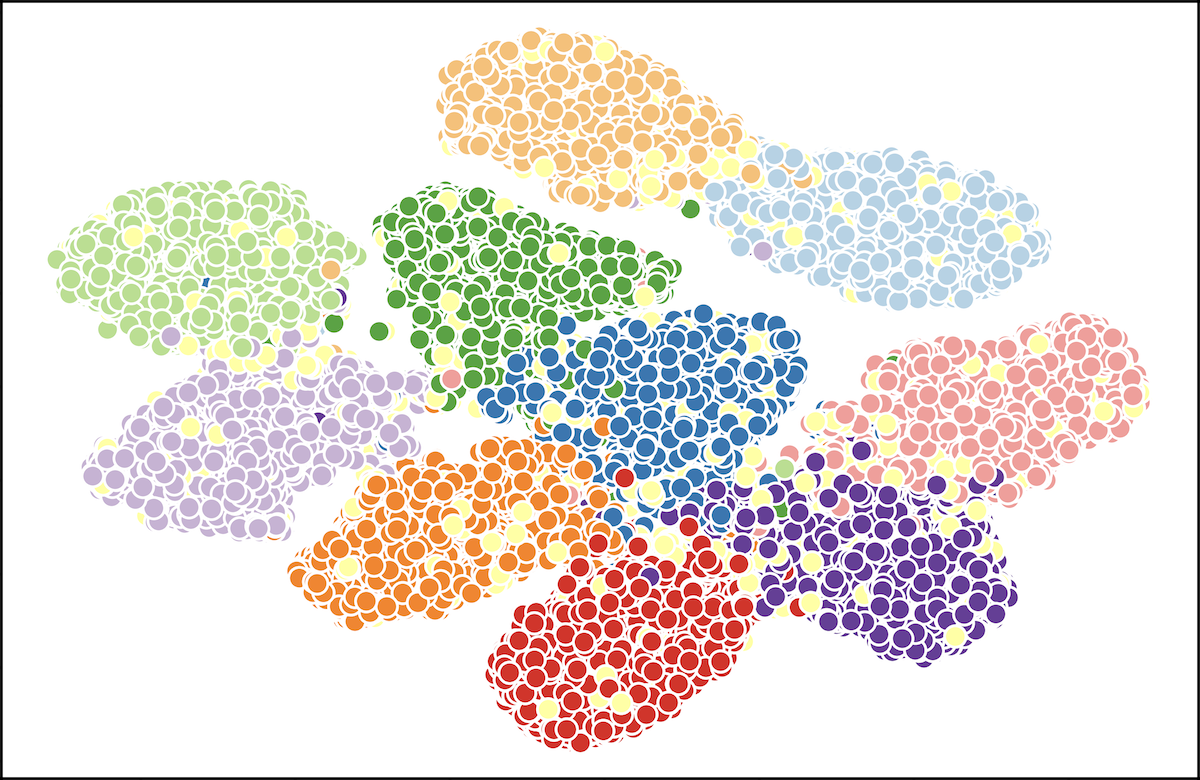
\includegraphics[width=0.32\textwidth]{src/wcl2-cifar10-1.png}}
\subfigure[P=30\%, 12000 samples]{
\label{Fig.sub.a2}
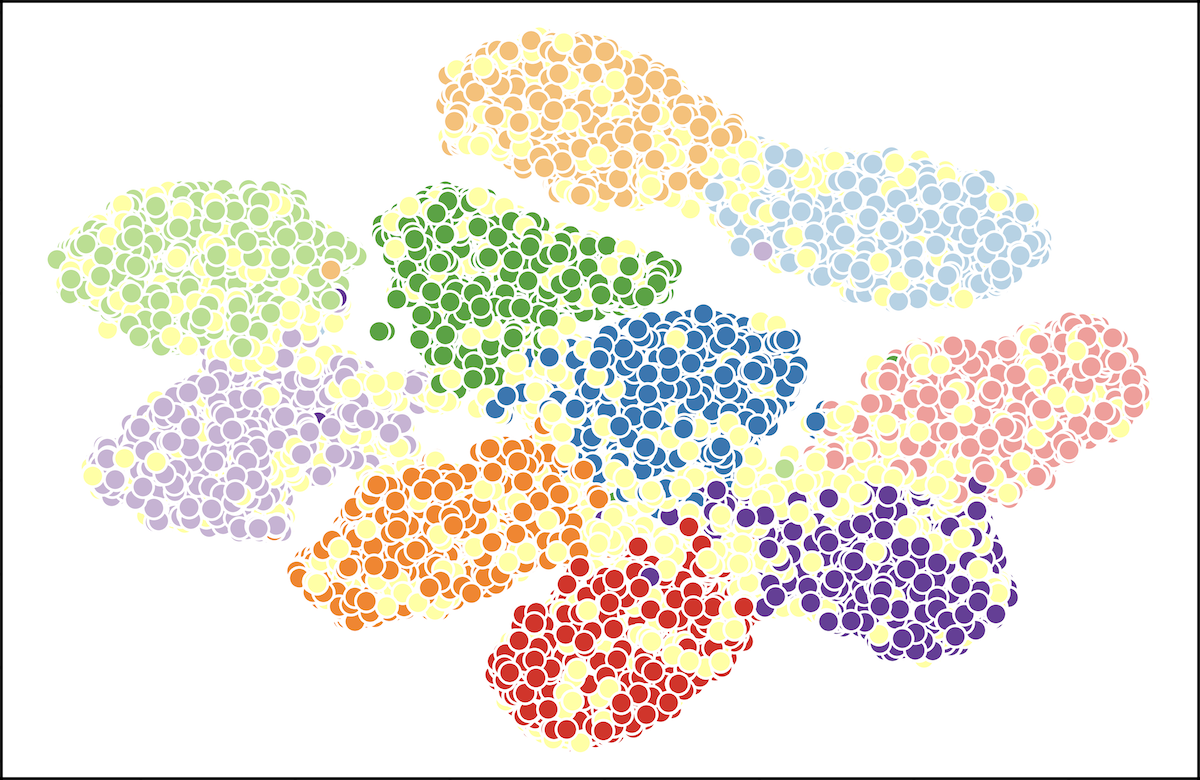
\includegraphics[width=0.32\textwidth]{src/wcl2-cifar10-3.png}}
\subfigure[P=50\%, 20000 samples]{
\label{Fig.sub.a1}
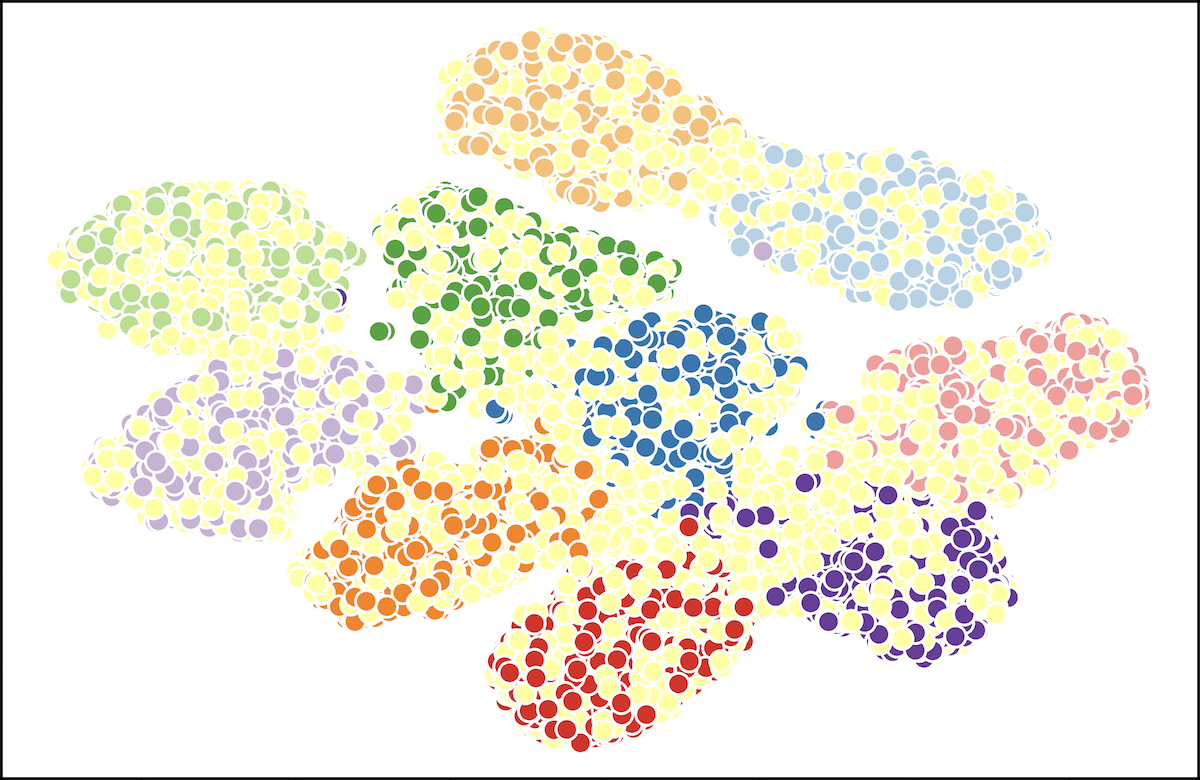
\includegraphics[width=0.32\textwidth]{src/wcl2-cifar10-5.png}}
\caption{WCL tune selection percentage. The first row we use weighted sampling method, the second row we use EGDIS based method.}
\label{Fig.wclcifar10}
\end{figure}

Therefore, we combined both WCL and EGDIS selected boundary samples and proposed the method BWCL. Compared with EGDIS, our BWCL can both get the similar score distribution as well as recover the shape of blobs. However, due to randomness during selection, we cannot guarantee to select the same datasets each time. This makes the classification accuracy unstable for machine learning models. We plotted the score distributions in Figure \ref{Fig.wclcifar10-dis}. We found that the score distribution of WCL is similar with the score distribution of the whole dataset in Figure \ref{Fig.clscores} while by selecting similar amount of samples, BWCL is similar with EGDIS in Figure \ref{Fig.egdiscifar10.a3}.

\begin{figure}[H]
\centering  
\subfigure{
\label{Fig.sub.a1}
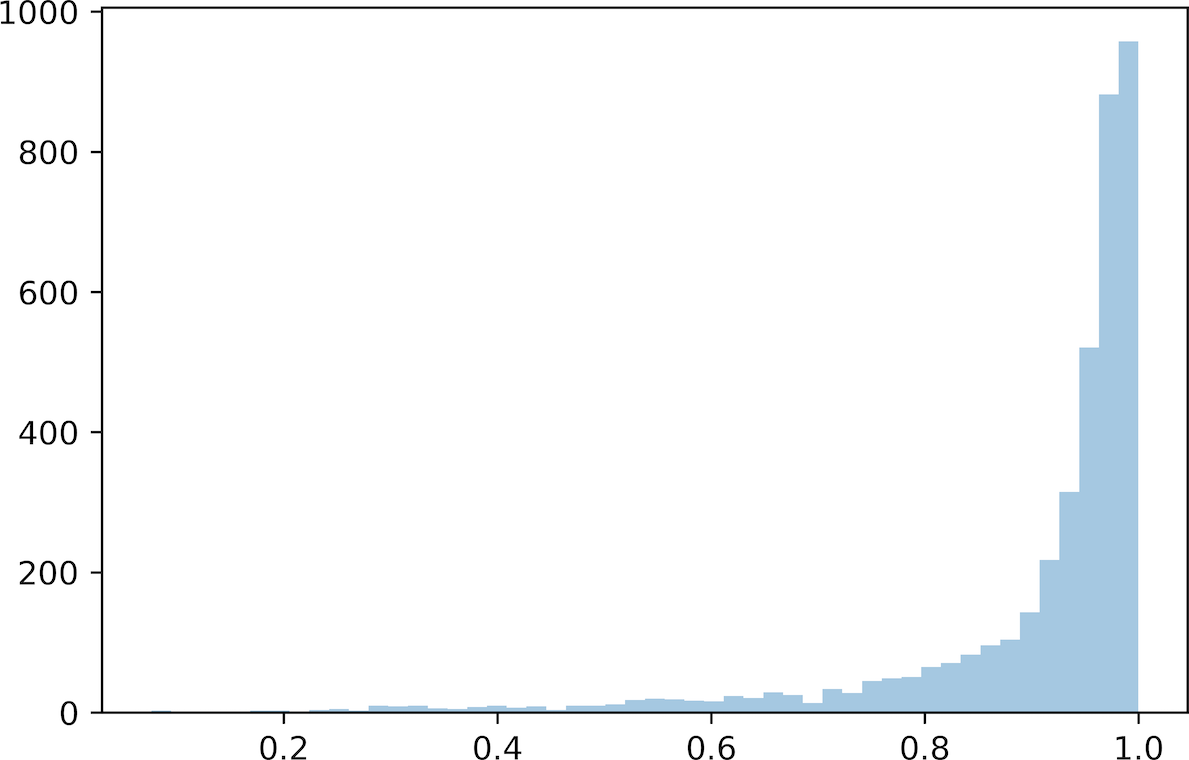
\includegraphics[width=0.32\textwidth]{src/wcl-cifar10-1-scoredis.png}}
\subfigure{
\label{Fig.sub.a2}
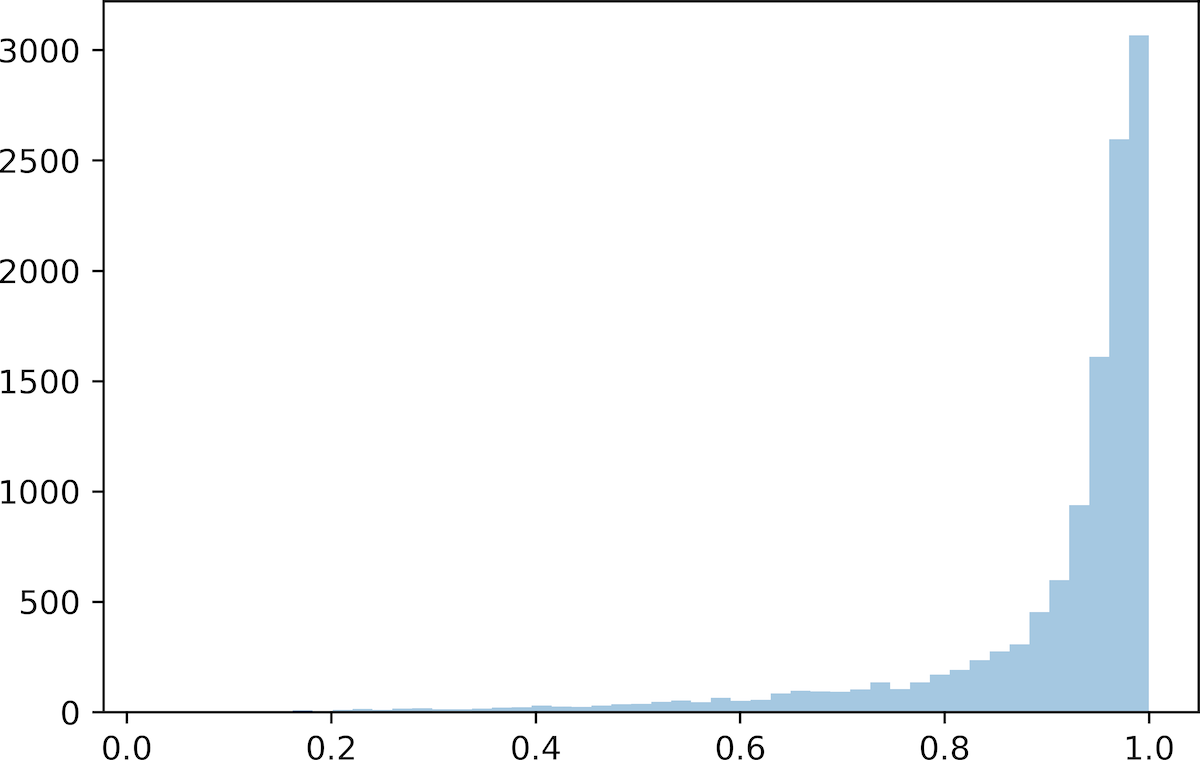
\includegraphics[width=0.32\textwidth]{src/wcl-cifar10-3-scoredis.png}}
\subfigure{
\label{Fig.sub.a1}
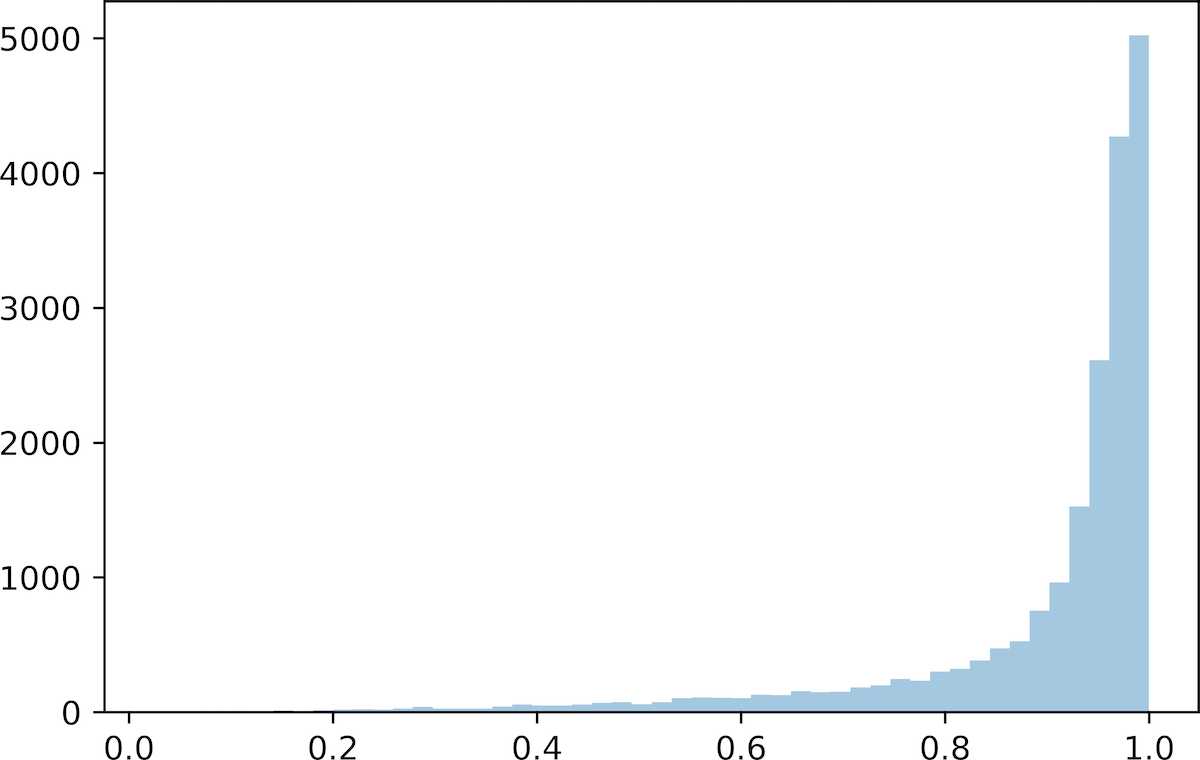
\includegraphics[width=0.32\textwidth]{src/wcl-cifar10-5-scoredis.png}}

\setcounter{subfigure}{0}
\subfigure[P=10\%, 4000 samples]{
\label{Fig.sub.a1}
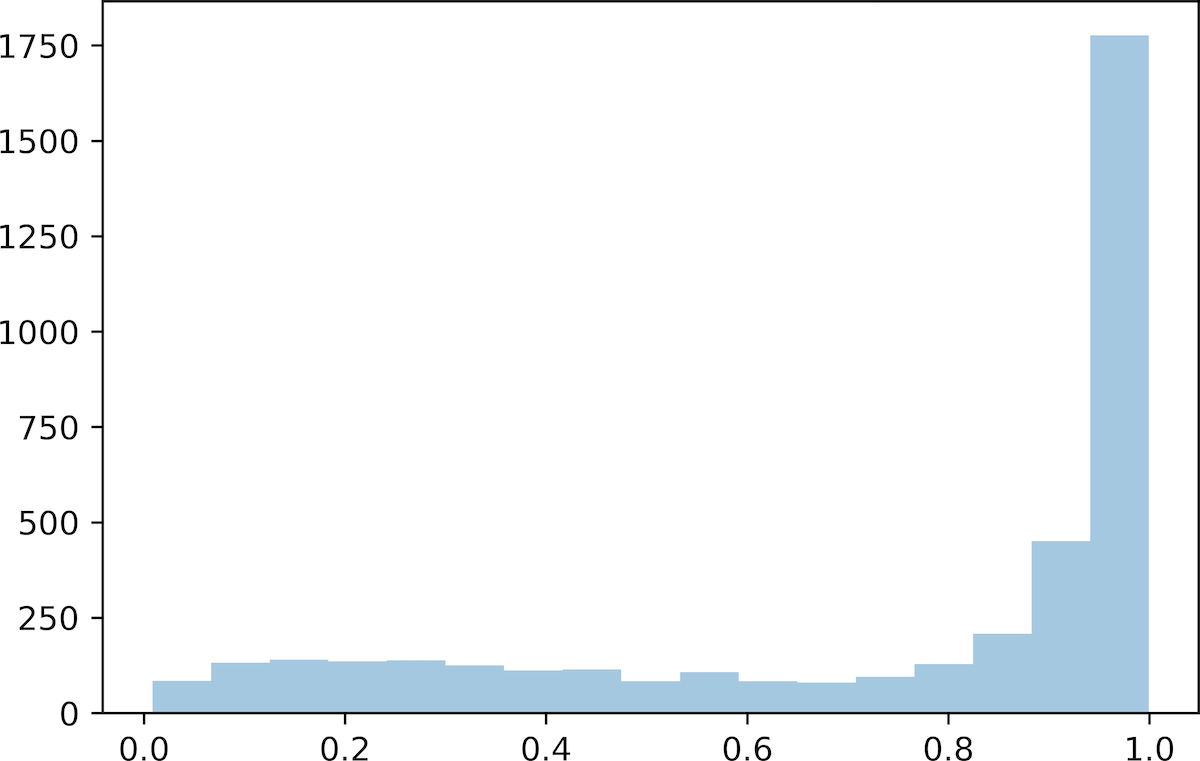
\includegraphics[width=0.32\textwidth]{src/bwcl-cifar10-1-scoredis.png}}
\subfigure[P=30\%, 12000 samples]{
\label{Fig.sub.a2}
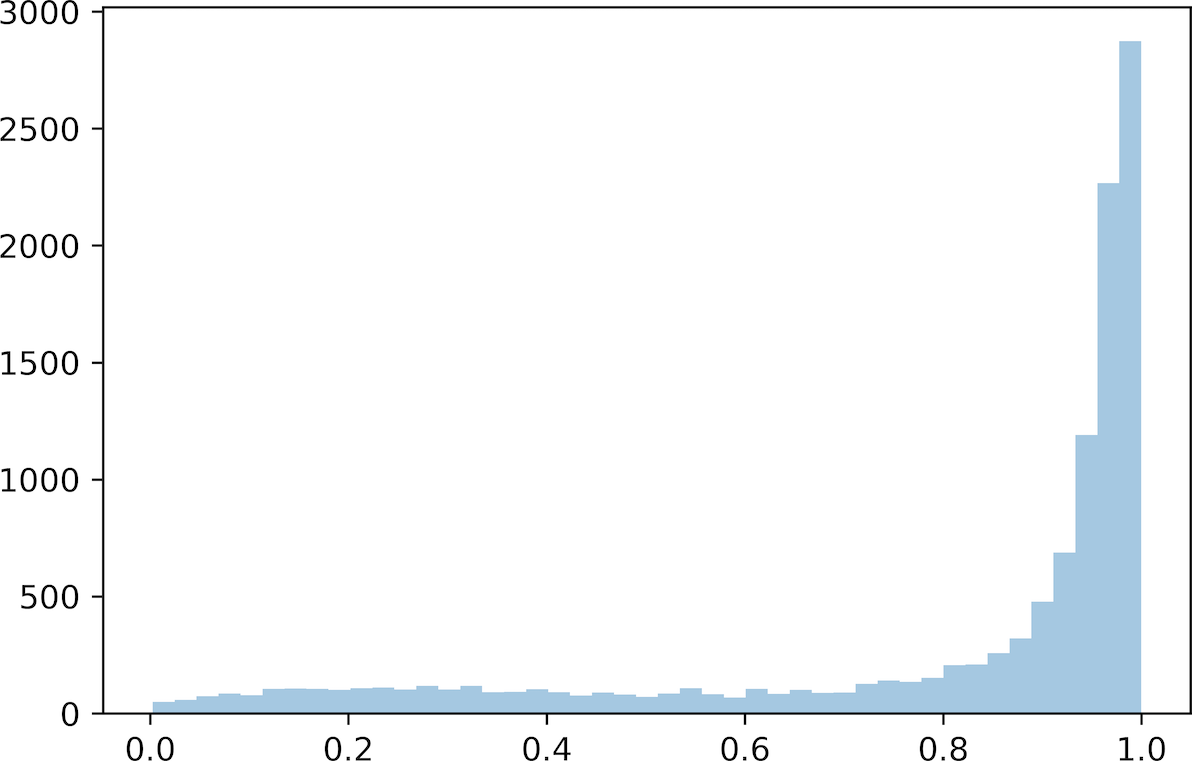
\includegraphics[width=0.32\textwidth]{src/bwcl-cifar10-3-scoredis.png}}
\subfigure[P=50\%, 20000 samples]{
\label{Fig.sub.a1}
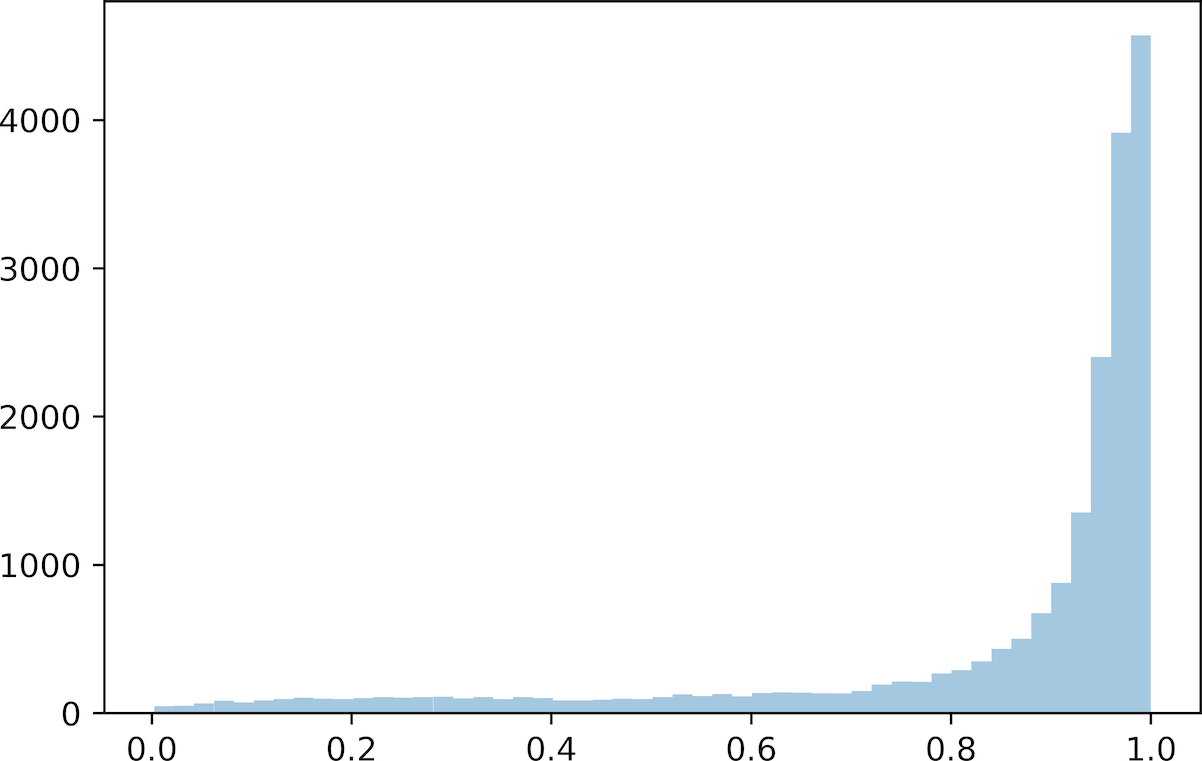
\includegraphics[width=0.32\textwidth]{src/bwcl-cifar10-5-scoredis.png}}
\caption{WCL tune selection percentage. The first row we use weighted sampling method, the second row we use EGDIS based method.}
\label{Fig.wclcifar10-dis}
\end{figure}


\section{Experiment 3: Logistic Regression}
\label{lr}

For more comprehensive evaluation results and inspired by \cite{Istrate2019}, we manually synthesised two CIFAR100 subsets and fill in the classification gap between CIFAR10 and CIFAR100. Between 10 classes to 90 classes with gap 10, we choose to build 9 subsets with by selecting the samples from required number of classes. For each required classes, we randomly do the job 5 times and trained them to convergence with logistic regression model. The boxplot is shown in Figure \ref{Fig.logistic_subsets}. We choose 40 classes and 20 classes as the number of our extra synthesised datasets, with LR test accuracy: 0.78925 and 0.853. They have 8,028 samples and 16042 samples. Then we repeated the feature compression process described before to fine-tuning the selected subsets and compress the extracted features. The final test accuracy is 0.8065 and 0.8745 respectively. In our reported accuracy below, we use CIFAR20 and CIFAR40 to refer to these synthesised datasets.

 \begin{figure}[H]
 \centering
 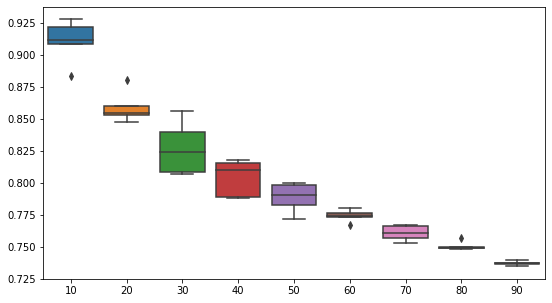
\includegraphics[width=0.8\textwidth]{src/subsets.png}
 \caption{The test set accuracies of CIFAR100 subsets. Horizontal axis is the number of classes selected. Vertical axis is the accuracy score. For each selection, we randomly choose the classes for five times and report the accuracy with logistic regression model.}
 \label{Fig.logistic_subsets}
 \end{figure}
 
 Our first discovery is that it is hard to select right amount of subsets with POP because the number of samples with weakness 128 is very low for all datasets except CIFAR10. Even for threshold 1, the number of pure inner is still low. Therefore, it is not good to choose samples with weakness < 128. From our experiment, we found that the reduction rate for EGDIS is good enough. Therefore, we make POP, CL, WCL and BWCL to select the same amount of samples as EGDIS. For POP, we ranked samples based on weakness and select from low to high. Therefore, we can have a fair comparison of their classification performance. The POP weakness distributions are shown in Figure \ref{Fig.pop_count}.
 
 \begin{figure}
\centering  
\subfigure[CIFAR10, 40000 samples]{
\label{Fig.sub.a1}
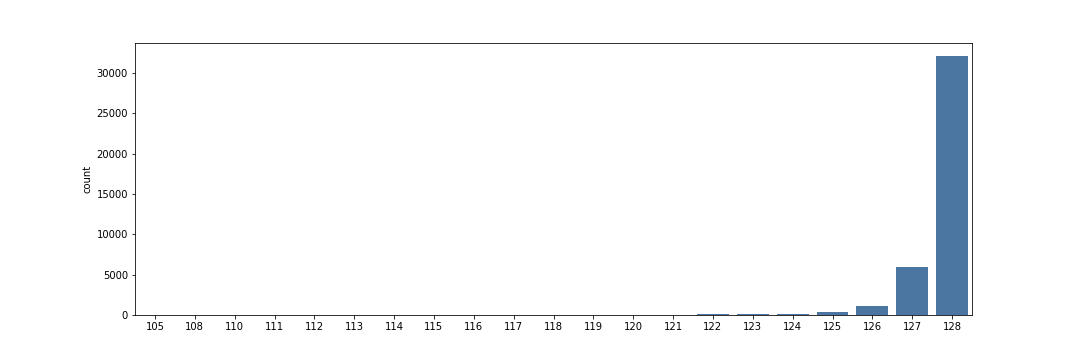
\includegraphics[width=0.4\textwidth]{src/pop-cifar10-count.png}}
\subfigure[CIFAR20, 8028 samples]{
\label{Fig.sub.a2}
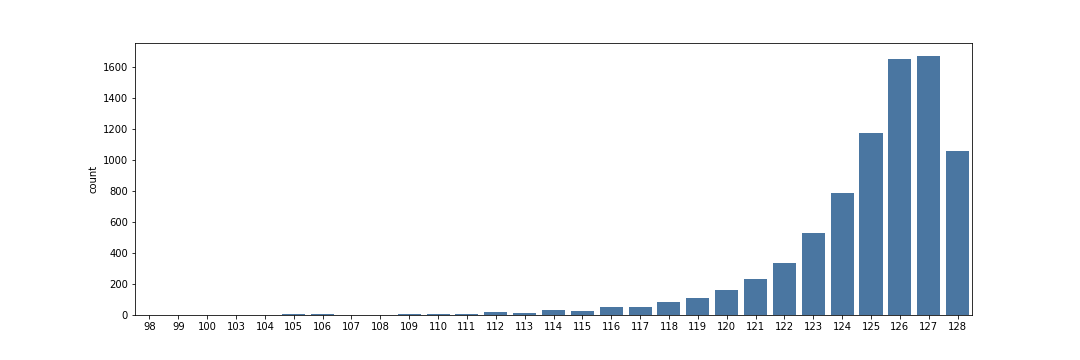
\includegraphics[width=0.4\textwidth]{src/pop-cifar20-count.png}}
\subfigure[CIFAR40, 16042 samples]{
\label{Fig.sub.a1}

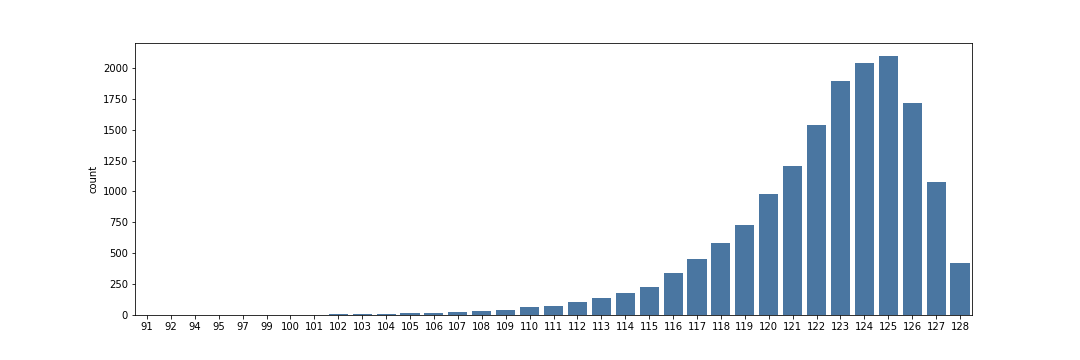
\includegraphics[width=0.4\textwidth]{src/pop-cifar40-count.png}}
\subfigure[CIFAR100, 40000 samples]{
\label{Fig.sub.a1}
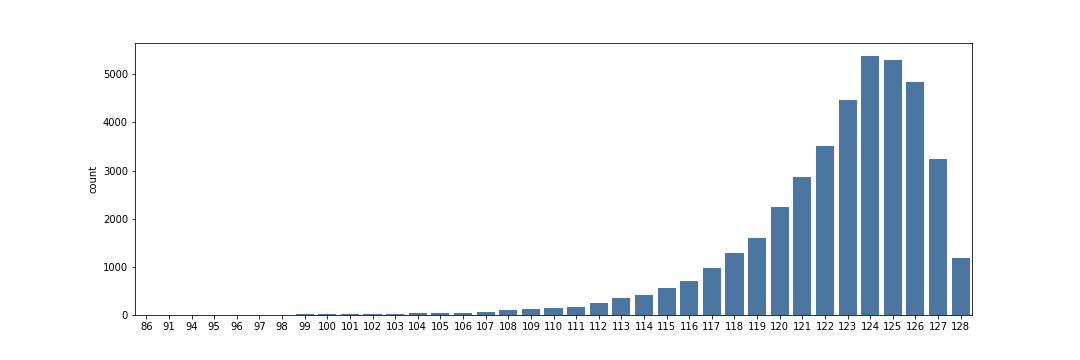
\includegraphics[width=0.4\textwidth]{src/pop-cifar100-count.png}}
\caption{POP with 4 datasets.}
\label{Fig.pop_count}
\end{figure}

For the five algorithms, we performed the selection process 12 times and reported the average accuracy with logistic regression model. The relative accuracy is recorded in Table \ref{lg_acc}. We can see that the retention rate is increasing with the classification difficulty of the datasets. POP and EGDIS perform better with simpler dataset such as CIFAR10. For EGDIS, it even achieved an accuracy increase. We think this is because with selected boundary and dense samples only, the overfitting problem is reduced. However, the performances of WCL and BWCL are more stable than EGDIS. Their relative accuracy decreases slowly just like POP. Among all three classification score based algorithms, BWCL is more capable of dealing with harder datasets. We believe the reason is that BWCL can maintain the EGDIS selected boundary and the self-adaptive selection manner of WCL.
 
\begin{table}[H]
    \centering
    \begin{tabular}{|l|l|l|l|l|l|l|}
    \hline
        Datasets & Retention Rate  & POP & EGDIS & CL & WCL & BWCL \\ \hline
        CIFAR10 & 14.915\% & 100.00\% & \textbf{100.04}\% & 99.74\% & 99.96\% & 99.91\% \\ \hline
        CIFAR20 & 16.67\% & \textbf{99.94}\% & 99.01\% & 99.57\% & 99.31\% & 99.43\% \\ \hline
        CIFAR40 & 21.09\% & \textbf{99.64}\% & 98.92\% & 99.09\% & 99.46\% & 99.63\% \\ \hline
        CIFAR100 & 31.48\% & 99.38\% & 97.78\% & 98.78\% & 99.46\% & \textbf{99.49}\% \\ \hline
    \end{tabular}
    \caption{Logistic Regression test set relative accuracy by averaging 12 runs}
    \label{lg_acc}
\end{table}

 We should notice that the average relative accuracy of BWCL is not the best value. We tuned the maximum proportion of boundary samples from 0.1 to 0.4 with step 0.1 and trained them 3 times each. In Figure \ref{Fig.logistic_relativeacc.a2}, we reported the relative accuracy in plot. It is clear that for simpler datasets, we should choose less hard examples. For harder datasets, we should choose more boundary samples. 

\begin{figure}[H]
\centering  
\subfigure[Relative Accuracy]{
\label{Fig.sub.a1}
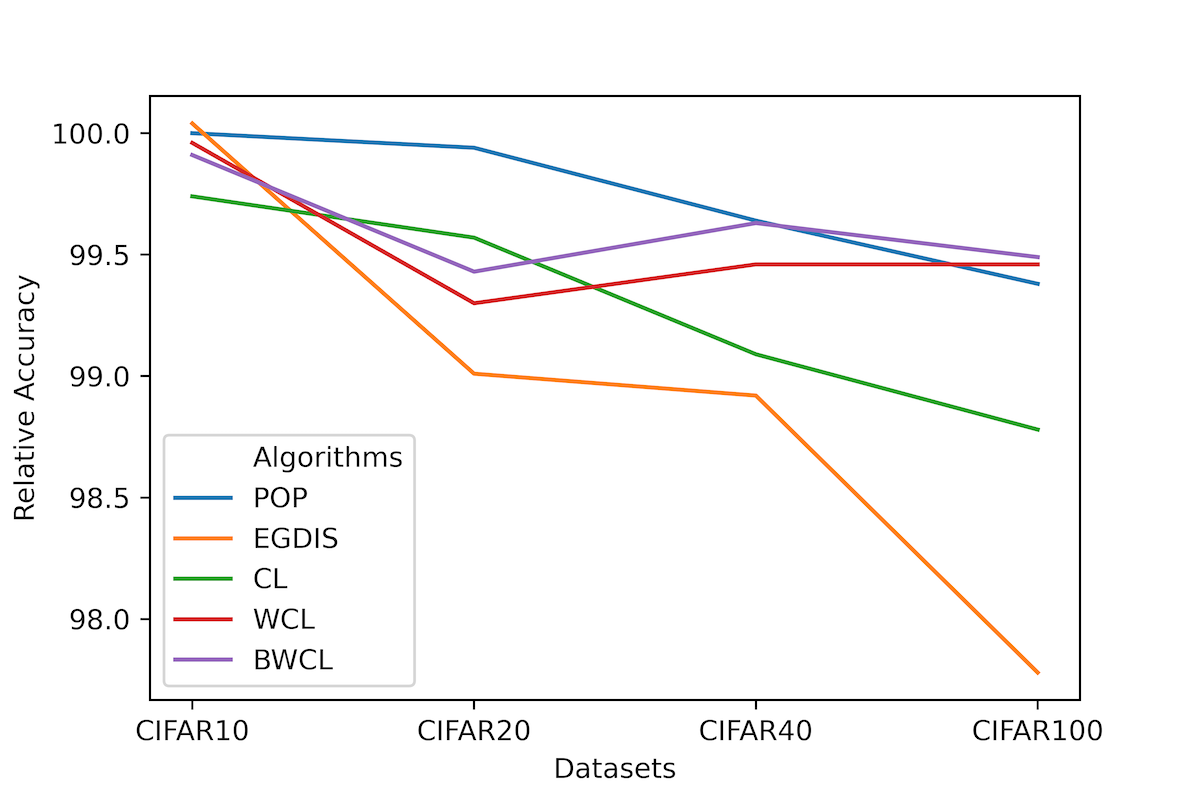
\includegraphics[width=0.45\textwidth]{src/lg_relative.png}}
\subfigure[Relative Accuracy of BWCL by tuning maximum boundary proportion]{
\label{Fig.logistic_relativeacc.a2}
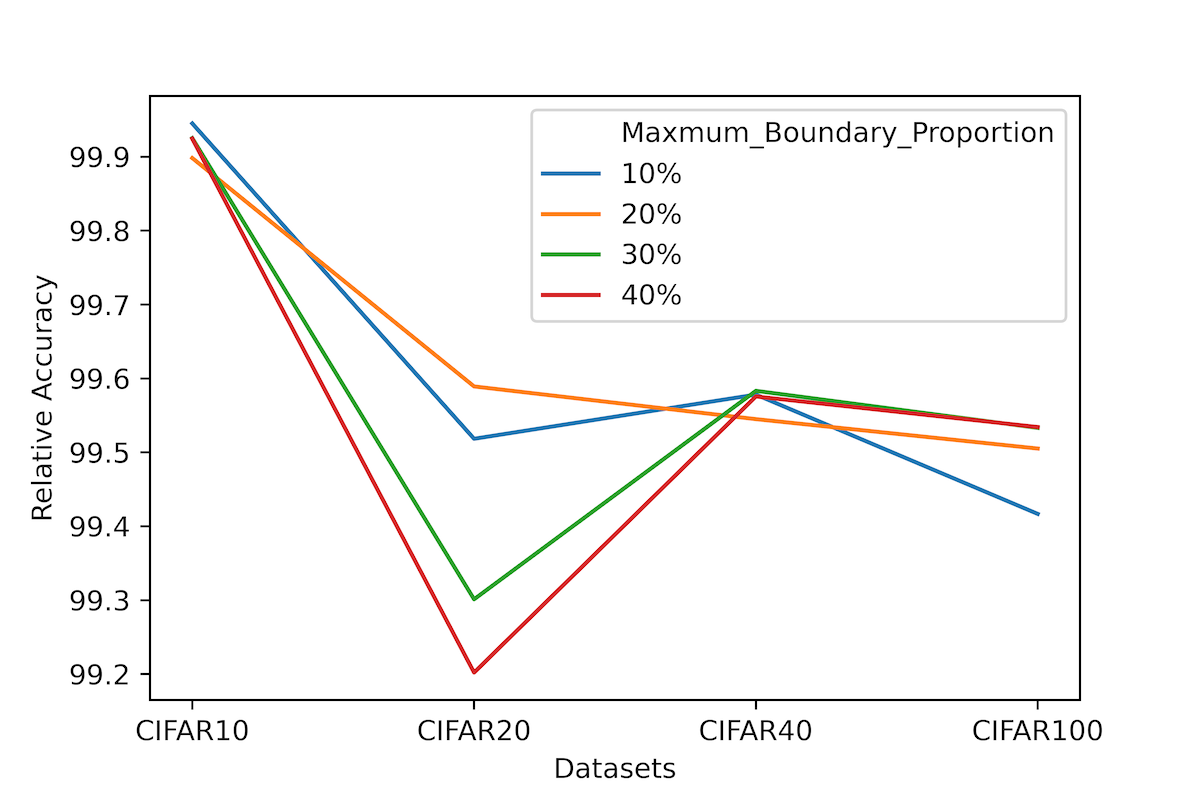
\includegraphics[width=0.45\textwidth]{src/bwcl_relative.png}}
\caption{Relative Accuracy of data reduction algorithms}
\label{Fig.logistic_relativeacc}
\end{figure}

We took a further analysis for BWCL, by varying the proportion of samples selected relative to the number of samples selected by EGDIS. We fixed the maximum boundary proportion to 0.4. The relative accuracy is reported in Figure \ref{Fig.logistic_subsets}. We found that the quality of the extracted features are so good that the test set samples are classified easily. This means that the results from logistic regression may not transfer to CNN experiments well but this provide us a good start.

\begin{figure}[H]
 \centering
 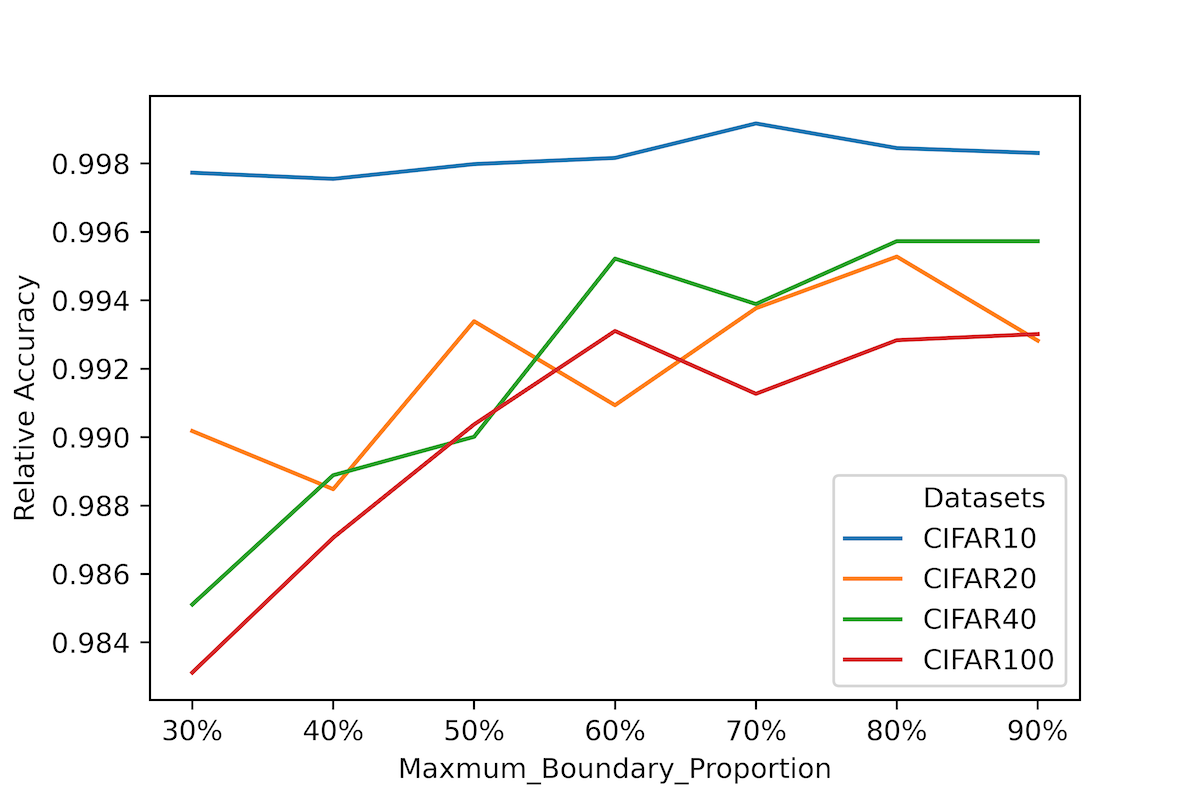
\includegraphics[width=0.8\textwidth]{src/bwcl_relative_size04.png}
 \caption{The BWCL test set accuracies. Averaged with 3 individual runs. The threshold is 10\%. Horizontal axis is the percentage of samples selected, in term of EDGIS selected samples. Vertical axis is the accuracy score.}
 \label{Fig.logistic_subsets}
 \end{figure}

\section{Experiment 4: Data Reduction for CNN}
\label{CNN}
We trained the network densenet101, three times, with learning rate 0.1 (150 epochs), 0.01 (100 epochs) and 0.001 (100 epochs). First we trained the network with the same selection configuration as logistic regression and reported the classification accuracy in Table \ref{CNN_accs}. 

\begin{table}[H]
    \centering
    \begin{tabular}{|l|l|l|l|l|l|l|}
    \hline
        Datasets & Retention Rate  & POP & EGDIS & CL & WCL & BWCL \\ \hline
        CIFAR10 & 14.915\% & 86.80\% & 85.18\% & 86.71\% &\textbf{88.36}\% & 86.75\% \\ \hline
        CIFAR20 & 16.67\% & 59.93\% & 61.43\% & \textbf{70.96}\% & 69.34\% & 64.67\% \\ \hline
        CIFAR40 & 21.09\% & 63.99\% & 63.89\% & \textbf{75.77}\% & 71.36\% & 70.65\% \\ \hline
        CIFAR100 & 31.48\% & 75.24\% & 73.74\% & 82.72\% & \textbf{83.23}\% & 81.69\% \\ \hline
    \end{tabular}
    \caption{CNN test set relative accuracy}
    \label{CNN_accs}
\end{table}

First of all, we found that POP and EGDIS selected samples are not suitable for neural network. The network cannot extract good features from these images thus the relative accuracy is much lower than expected. Second, classification score based algorithms can achieve relatively higher accuracy. In particular, for datasets with less per-class samples, CL is better. For datasets with more per-class samples, WCL is better. However, BWCL performs worse  than expected. We believe that this is because we evaluated the classification scores with NasNetLarge, who has better extraction power than DenseNet. We just contains too much hard examples so the network cannot handle the training samples well. We proposed another hypothesis that if the network could learn these hard samples well, then it should be able to achieve higher classification accuracy based on the hard-example mining method described before. 

\begin{figure}[H]
\centering  
\subfigure[Relative Accuracy]{
\label{Fig.sub.a1}
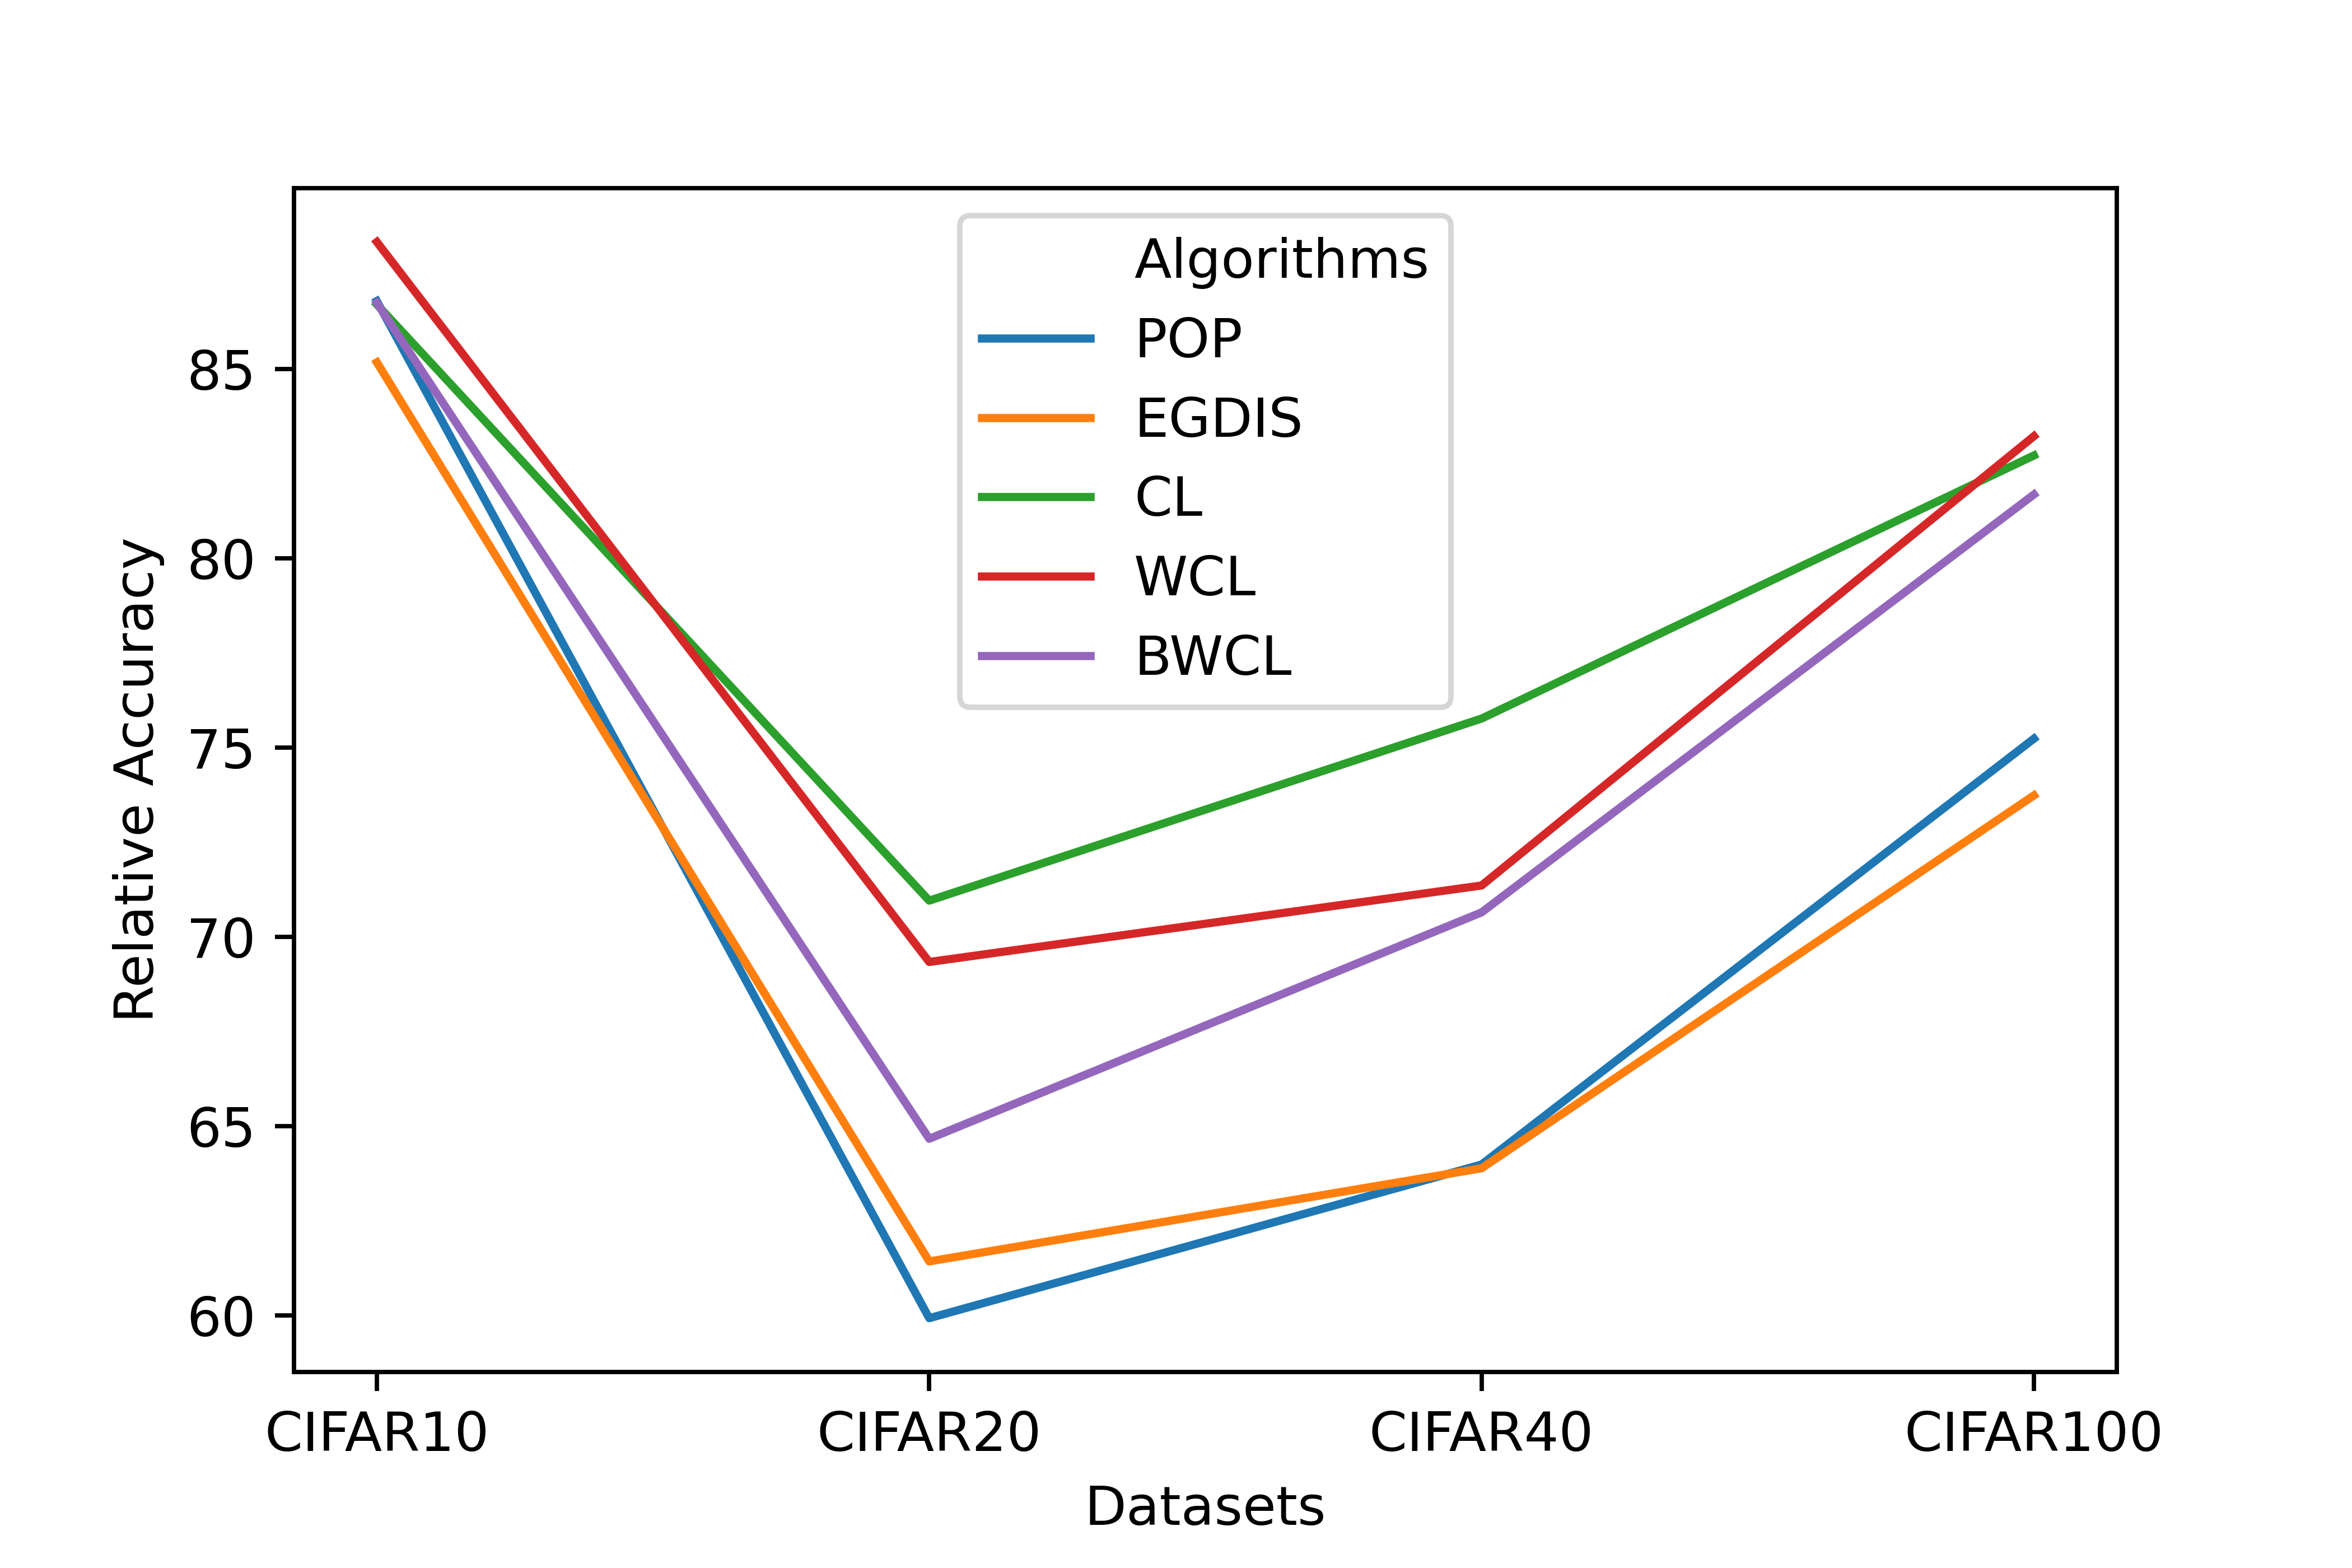
\includegraphics[width=0.45\textwidth]{src/cnn-alg-relative.png}}
\subfigure[Relative Accuracy of BWCL by tuning maximum boundary proportion]{
\label{Fig.sub.a2}
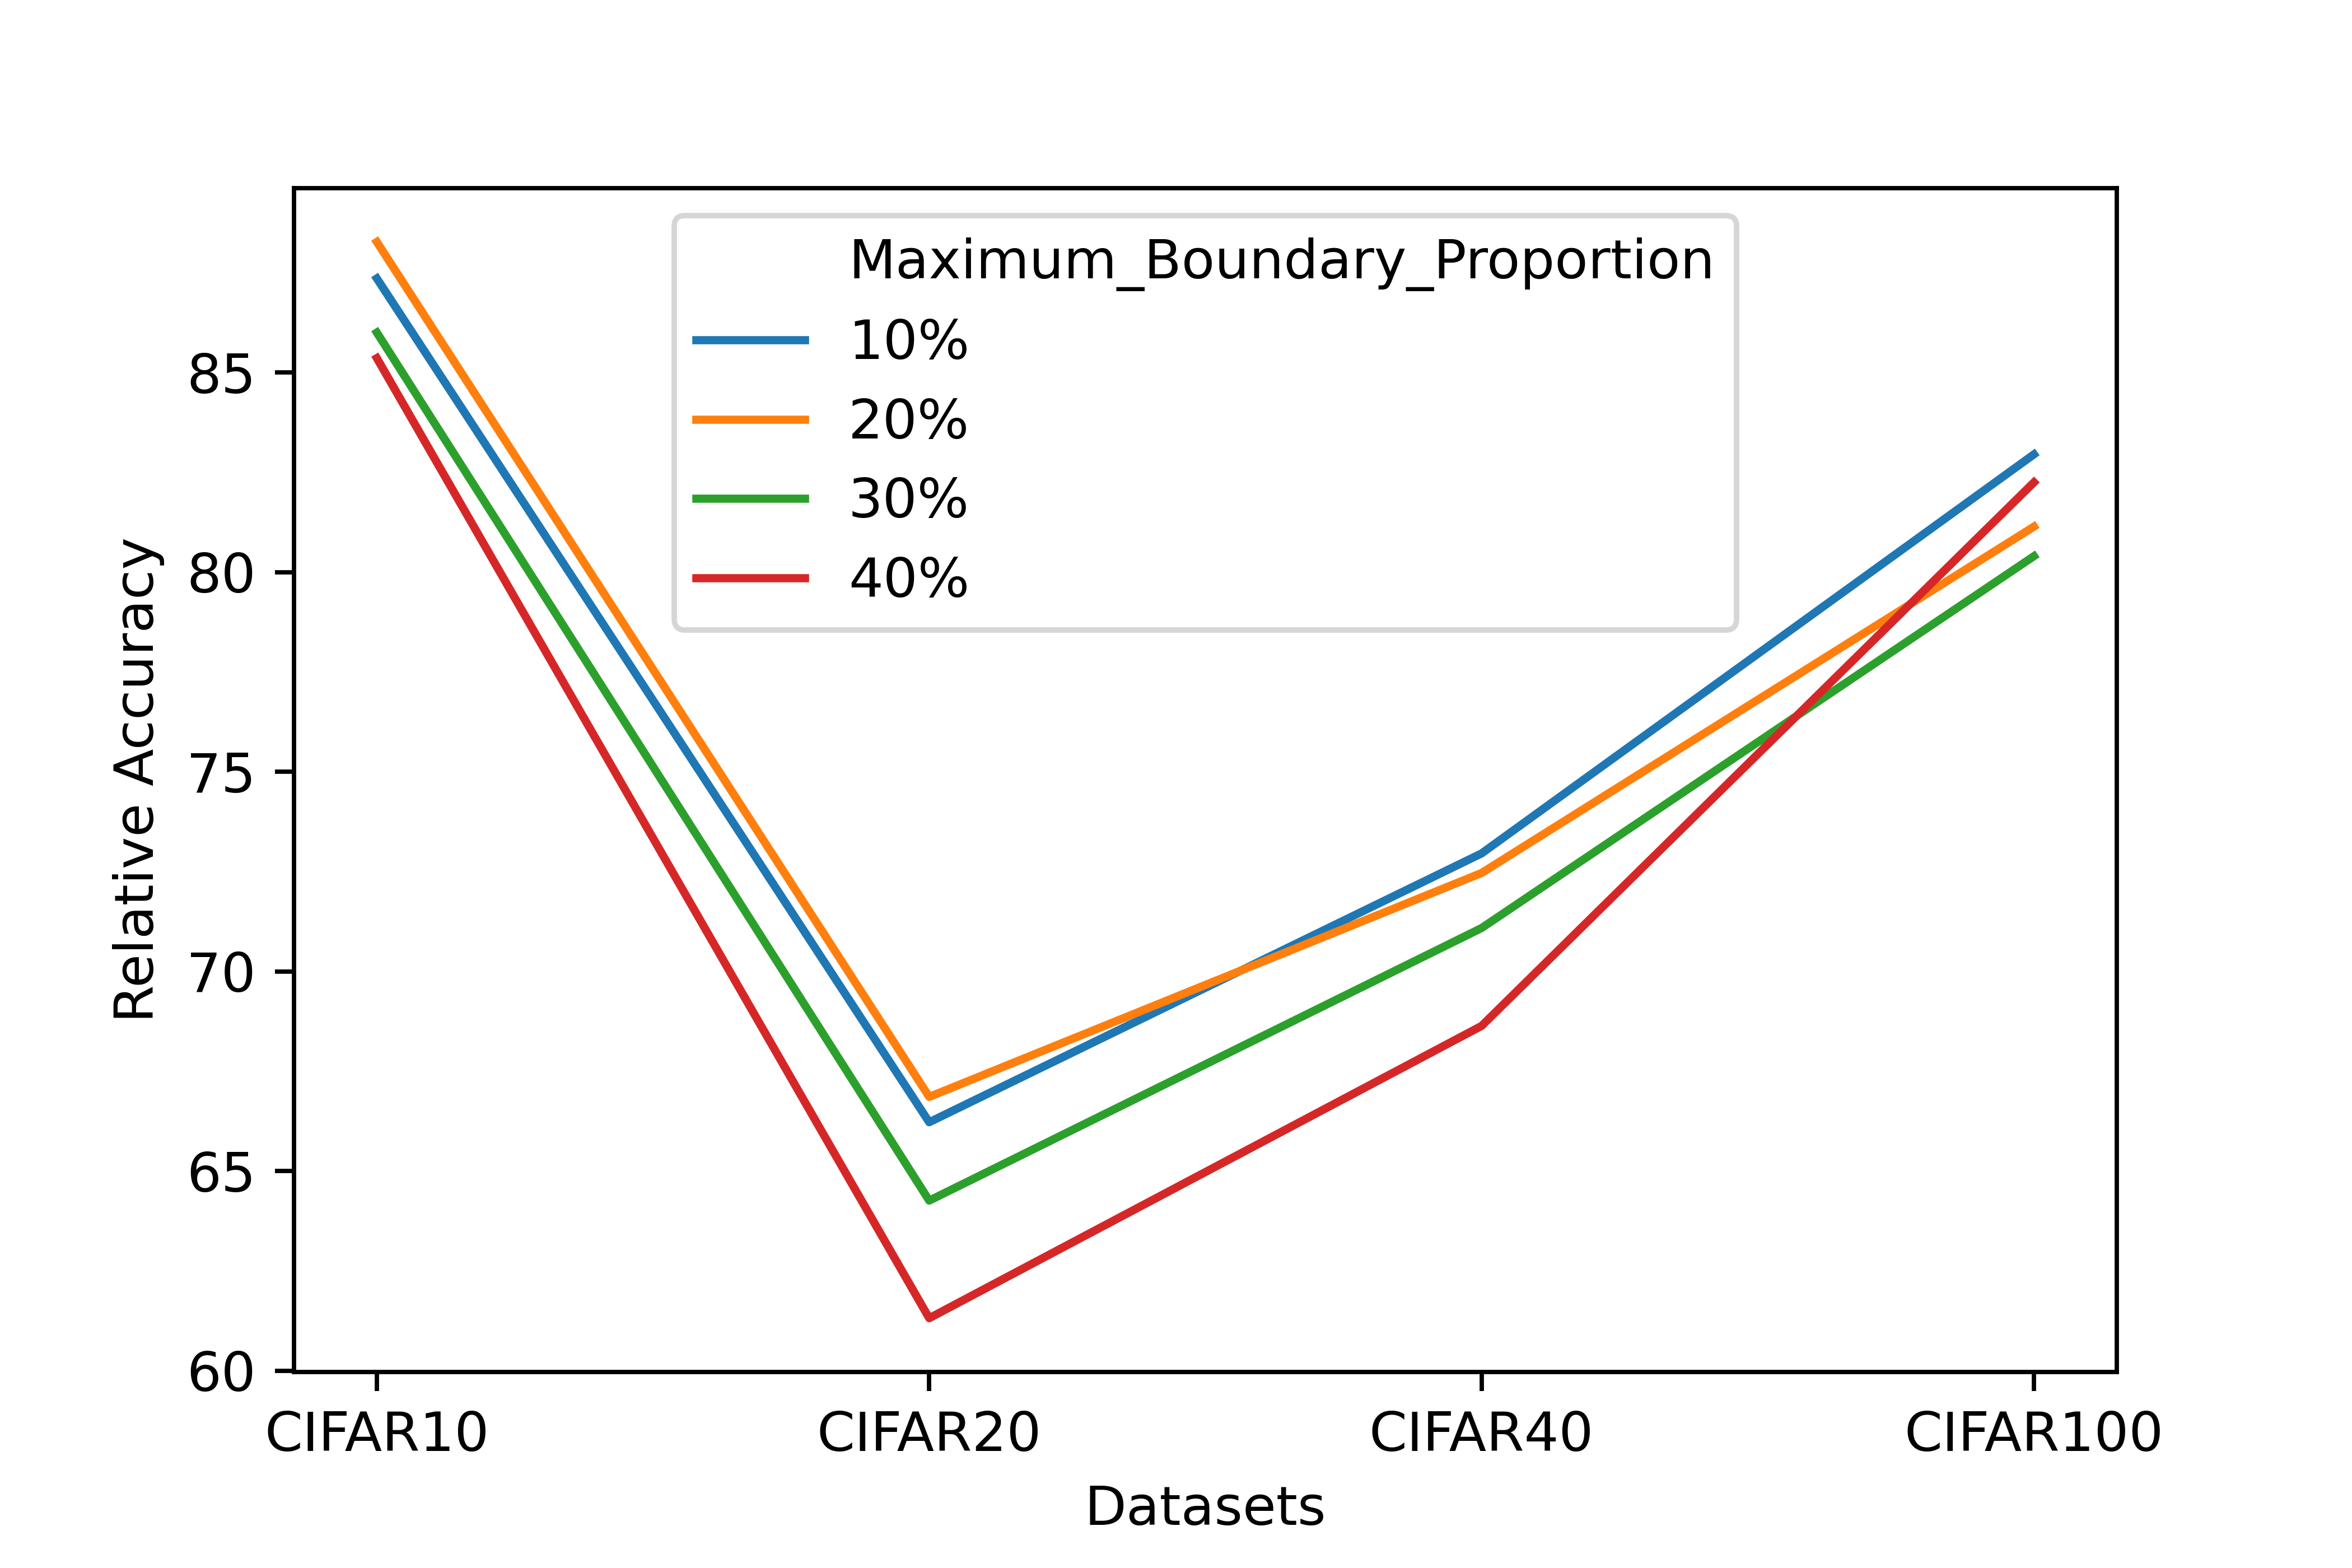
\includegraphics[width=0.45\textwidth]{src/cnn-bwcl-relative.png}}
\caption{Relative Accuracy of data reduction algorithms}
\label{Fig.logistic_relativeacc}
\end{figure}

We took a closer look at the training curve of the first training stage to analysis the convergence speed. For all datasets, CL selected samples can help the network to converge faster. 

\begin{figure}[H]
\centering  
\subfigure[CIFAR10]{
\label{Fig.sub.a1}
\includegraphics[width=0.45\textwidth]{src/trend_cifar10.png}}
\subfigure[CIFAR100]{
\label{Fig.sub.a2}
\includegraphics[width=0.45\textwidth]{src/trend_cifar100.png}}

\subfigure[CIFAR20]{
\label{Fig.sub.a2}
\includegraphics[width=0.45\textwidth]{src/trend_cifar20.png}}
\subfigure[CIFAR40]{
\label{Fig.sub.a2}
\includegraphics[width=0.45\textwidth]{src/trend_cifar40.png}}
\caption{The training trend of four datasets by selecting the same amount of samples as EGDIS, of the first 150 epochs}
\label{Fig.training_trend}
\end{figure}
